% Created 2022-03-21 Mon 23:55
% Intended LaTeX compiler: pdflatex
\documentclass[9pt]{article}
\usepackage[hidelinks]{hyperref}
\usepackage[left=3cm, right=3cm, top=2cm, bottom=2cm]{geometry}
\usepackage{amsmath}
\usepackage{titlesec}
\usepackage{minted}
\setcounter{secnumdepth}{12}
\setcounter{tocdepth}{2}
\titleformat{\paragraph}
{\normalfont\normalsize\bfseries}{\theparagraph}{1em}{}
\titlespacing*{\paragraph}
{0pt}{3.25ex plus 1ex minus .2ex}{1.5ex plus .2ex}
\usepackage{indentfirst}
\setlength{\parindent}{1em}
\setlength{\parskip}{1em}
\usepackage[export]{adjustbox}
\raggedbottom
\usepackage{float}
\clearpage
\usepackage{longtable}
\usepackage{array}
\usepackage{multirow}
\newcolumntype{C}[1]{>{\centering\arraybackslash}p{#1}}
\usepackage{gensymb}
\usepackage{graphicx}
\usepackage{tikz}
\usepackage{tikz-feynman}
\usetikzlibrary{arrows.meta, decorations.pathreplacing, decorations.markings, decorations.pathmorphing}
\tikzset{snake it/.style={decorate, decoration=snake}}
\usepackage{multicol}
\usepackage{tcolorbox}
\setlength{\columnsep}{0.1cm}
\setlength{\columnseprule}{0.5pt}
\def\columnseprulecolor{\color{white}}
\renewcommand\fbox{\fcolorbox{lightgray}{white}}
\usepackage{framed}
\usepackage{xcolor}
\definecolor{CodeGray}{gray}{0.40}
\definecolor{RuleGray}{gray}{0.40}
\usepackage{xpatch}
\let\oldsection\section
\renewcommand\section{\clearpage\oldsection}
\usepackage{fancyhdr}
\pagestyle{fancy}
\fancyhf{}
\pagestyle{fancy}
\rhead{\emph{Alexander F. Neville}}
\lhead{AQA A-Level Computer Science}
\rfoot{\thepage}
\lfoot{\leftmark}
\renewcommand{\headrulewidth}{1pt}
\renewcommand{\footrulewidth}{1pt}
\xpretocmd\headrule{\color{lightgray}}{}{\PatchFailed}
% \xpretocmd\footrule{\color{lightgray}}{}{\PatchFailed}
\usepackage{etoolbox}
\makeatletter
\patchcmd{\footrule}
{\if@fancyplain}
{\color{lightgray}\if@fancyplain}
{}
{}
\makeatother
\usepackage{amsmath}
\usepackage{amsmath}
\usepackage{amsmath}
\usepackage{amsmath}
\usepackage{amsmath}
\author{Alexander Neville}
\date{\today}
\title{Computer Science Notes}
\hypersetup{
 pdfauthor={Alexander Neville},
 pdftitle={Computer Science Notes},
 pdfkeywords={},
 pdfsubject={},
 pdfcreator={Emacs 27.1 (Org mode 9.6)}, 
 pdflang={English}}
\begin{document}

\maketitle
\tableofcontents

\thispagestyle{empty}
\begin{figure}[H]
\centering
% \includegraphics[width=0.9\textwidth,keepaspectratio,frame]{./images/}
\end{figure}
\newpage
%inner square side length
\def\a{3.0}
%outer square side length
\def\b{5.0}
% x displacement of back squares
\def\dx{0.8}
% y displacement of back squares
\def\dy{0.5}
\def\lx{1.0}
\def\ly{1.0}
% round corner correction
\def\dr{0.02}
% \tableofcontents

\section{Fundamentals of Programming}
\label{sec:org035610e}

An algorithm is a series of steps underlying every process including programs. An abstract view of any program/algorithm is \emph{input -> process -> output}.

\subsection{Pseudocode}
\label{sec:orga098029}

Rather than try and solve a problem while implementing a program, it can help to try and outline the solution in a abstract manner and then write the code to solve the problem. Pseudocode is a flexible method of planning an algorithm that is easier to read and understand, while keeping in the programming mindset. Pseudocode is written like a program, with data types, flow control, operators etc.

\subsubsection{Syntax}
\label{sec:org6145426}

\textbf{Comments:}

Anything following a \texttt{\#} symbol is a comment.

\textbf{Data Types:}

Pseudocode is not strongly typed so there is generally no need to specify the data type on initialisation. Pseudocode variables typically fall into these categories:

\begin{itemize}
\item \emph{integer} (any unbounded whole number)
\item \emph{real/float} (any number with a fractional part)
\item \emph{boolean} (a true/false variable)
\item \emph{character} (a single digit represented in ASCII or similar)
\item \emph{string} (more than one character in a row)
\end{itemize}

NB. all data-types will have a constructor eg. \emph{int(``2'')} or \emph{str(2)} for easy conversion.
NB. all iterable series in pseudocode are 1 based.

\textbf{Assignment:}

The \texttt{=} sign is often used. A left arrow \texttt{<-} is sometimes used to show the flow of data. Variable names are all lowercase, while constants are defined with uppercase identifiers.

\textbf{Operators:}

Like other languages, the symbols \texttt{*/-+} are used. In addition these rules tend to apply:

\begin{itemize}
\item Assignment operators are rarely used as they tend to obfuscate the step by step approach to problem solving; code is usually broken into \emph{input -> process -> output} cycle.
\item To raise a number to a certain power, this syntax is used: \texttt{x**n}, where \emph{x} is the base and \emph{n} in the exponent.
\end{itemize}

\textbf{Keyword Functions:}

Besides the symbolic operators there are a number of functions and statements built into pseudocode. Here are a few:

\begin{itemize}
\item \emph{div} (floor divide operator, returning a whole number)
\item \emph{mod} (find the remainder of a certain div operation)
\item \emph{length()} (find the length of a string)
\item \emph{string.substring(index, index)} (return the string found between inclusive indices)
\item \emph{string.find(substring)} (return the first index of substring if found, else return -1)
\item \emph{ord(``x'')} (find the ASCII value of a character)
\item \emph{chr(97)} (find the character associated with a number)
\end{itemize}

\textbf{Input and Output:}

Input can be taken by assigning the result of \texttt{USERINPUT} to an identifier. The \texttt{OUTPUT} statement can print data. \texttt{INPUT} is sometimes used when the is not necessarily entered by a person.

\begin{figure}[H]
\begin{minted}[ frame=single, framesep=8mm, rulecolor=RuleGray, baselinestretch=1.3, fontsize=\small, breaklines, fontfamily=tt]{text}
sensor_data <- INPUT
name <- USERINPUT

OUTPUT name, sensor_data
\end{minted}
\end{figure}

\subsubsection{Flow Control}
\label{sec:org4c26a6b}

Pseudocode can combine its syntax with flow control mechanisms to build more functional programs.

\textbf{Relational Operators:}

Pseudocode uses all the typical relational operators, eg. \emph{<=, >=, <, >}. In addition a single \emph{=} sign is used as a comparison operator as \texttt{<-} is typically used for assignment. The \texttt{<>} symbol is used as not equal to operator.

\textbf{Boolean Logic:}

\texttt{AND}, \texttt{OR} and \texttt{NOT} can be used to create logical statements.

\textbf{Conditional Statements:}

This is how a typical condition is constructed:

\begin{figure}[H]
\begin{minted}[ frame=single, framesep=8mm, rulecolor=RuleGray, baselinestretch=1.3, fontsize=\small, breaklines, fontfamily=tt]{text}
IF (condition) THEN

    ....

ELSE IF (condition) THEN

    ....

ENDIF
\end{minted}
\end{figure}

\textbf{Switch Statements:}

If multiple options are dependent on the value of a single variable, a switch statement can be used.

\begin{figure}[H]
\begin{minted}[ frame=single, framesep=8mm, rulecolor=RuleGray, baselinestretch=1.3, fontsize=\small, breaklines, fontfamily=tt]{text}
CASE variable of

    value:

        ....

    value:

        ....

ENDCASE
\end{minted}
\end{figure}

\textbf{Iteration:}

Predicated \emph{while} loops are constructed like this:

\begin{figure}[H]
\begin{minted}[ frame=single, framesep=8mm, rulecolor=RuleGray, baselinestretch=1.3, fontsize=\small, breaklines, fontfamily=tt]{text}
WHILE condition

    ....

ENDWHILE
\end{minted}
\end{figure}

\emph{Do while} loops are also a possibility, useful if code must run at least once.

\begin{figure}[H]
\begin{minted}[ frame=single, framesep=8mm, rulecolor=RuleGray, baselinestretch=1.3, fontsize=\small, breaklines, fontfamily=tt]{text}
REPEAT

    ....

UNTIL condition
\end{minted}
\end{figure}

If the number of iterations is know, a \emph{for} loop can be used

\begin{figure}[H]
\begin{minted}[ frame=single, framesep=8mm, rulecolor=RuleGray, baselinestretch=1.3, fontsize=\small, breaklines, fontfamily=tt]{text}
FOR variable <- value TO value STEP value

    ....

ENDFOR
\end{minted}
\end{figure}

\subsubsection{Data structures}
\label{sec:orgf5f5c7e}

Arrays are a collection type which are usually filled with data of one type and unite values under one identifier. Individual values can be accessed with indexing eg. \texttt{array[x]} will return the value at position \emph{x} along \emph{array}. Arrays may be multi-dimensional and values can be addressed like this: \texttt{array[x][y]}.

\subsubsection{Subroutines}
\label{sec:org2c4d115}

A subroutine is a named block of code within a program. A subroutine may perform an operation as in a \emph{procedure} or return a value to the main program as a \emph{function.} In pseudocode a subroutine can be defined and called like this:

\begin{figure}[H]
\begin{minted}[ frame=single, framesep=8mm, rulecolor=RuleGray, baselinestretch=1.3, fontsize=\small, breaklines, fontfamily=tt]{text}
SUB procedure

    ....

END SUB

SUB function(input)

    ....
    RETURN output

ENDSUB

procedure
data <- function(data)
\end{minted}
\end{figure}

\subsubsection{Files}
\label{sec:org4fd4c41}

To store data permanently, It must be written to a file on disk. A file contains \emph{records} (rows) with many \emph{fields}. Data can be read from a file like this:

\begin{figure}[H]
\begin{minted}[ frame=single, framesep=8mm, rulecolor=RuleGray, baselinestretch=1.3, fontsize=\small, breaklines, fontfamily=tt]{text}
OPEN file for reading
FOR line <- 1 TO num_lines

    record = READLINE(file, line)
    OUTPUT record[1], record[2], ...

ENDFOR
CLOSE file
\end{minted}
\end{figure}

\subsubsection{Exceptions}
\label{sec:orgb54f198}

To define behaviour for an error condition, exception handling can be used.

\begin{figure}[H]
\begin{minted}[ frame=single, framesep=8mm, rulecolor=RuleGray, baselinestretch=1.3, fontsize=\small, breaklines, fontfamily=tt]{text}
TRY

    ....

EXCEPT

    OUTPUT "there was an error"

ELSE

    OUTPUT "end of statement"

ENDEXCEPT
\end{minted}
\end{figure}

\section{Problem Solving and Theory of Computation}
\label{sec:orge84e200}
\subsection{Problem Solving}
\label{sec:org03baaf4}

Besides writing larger programs, computing has many applications involving smaller problems. A \emph{puzzle} is a problem that is solved by selecting the right inputs. This process can be performed computationally. The problem may be \emph{specific}, having a certain number of inputs (eg. 3), or \emph{general}, having \emph{n} number of inputs. These values can be used to calculate the efficiency of an algorithm.

\subsection{Strategies}
\label{sec:org943c561}

There are some common strategies for solving logic/computational problems:

\begin{itemize}
\item \emph{exhaustive}, can be described as systematic, is a \emph{brute-force} technique. The inputs are not selected intelligently, based on higher probability of solving the problem, but rather randomly or in some arbitrary order.
\item \emph{divide-and-conquer}, works best with partially solved puzzles, eg. sorted list. The number of inputs is repeatedly split and the more probable path is taken.
\end{itemize}

\subsection{Structured Programming}
\label{sec:org7f9497f}

In order to ease development and make maintainable programs, an algorithm is divided into smaller parts.

\subsubsection{Block Structure}
\label{sec:org3501181}

In block-structured languages, an algorithm can be broken down into the repeated use of just three structures:

\begin{itemize}
\item \emph{sequence} -  a block of code composed of one instruction after the other (single thread of execution)
\item \emph{selection} - the use of a conditional statement to execute certain sequences depending on an event
\item \emph{iteration} - the use of abstract \emph{jumps} to repeat a sequence of code
\end{itemize}

Modern programming languages use syntax elements to make these \emph{blocks} apparent. Curly brackets, \texttt{\{\},} or indentation and significant white space might be used to make code blocks visually distinct.

\subsubsection{Modularisation}
\label{sec:org0fca1cd}

An algorithm is repeatedly broken down into smaller parts until each can easily be implemented in a single \emph{sub-routine}, sometimes called a \emph{module}. This is called \emph{top-down} design. The advantages of this technique include:

\begin{itemize}
\item individual module/unit testing
\item reusable and distributable modules
\item many people can work on a project simultaneously
\end{itemize}

\subsubsection{Hierarchy Charts}
\label{sec:org4702830}

A hierarchy chart is a way of visualising how an algorithm is broken down. Each step may be a logical block or a sub-routine that has been programmed. A hierarchy chart does not describe the implementation of a problem, nor the control flow within each module.

\begin{figure}[H]
\centering
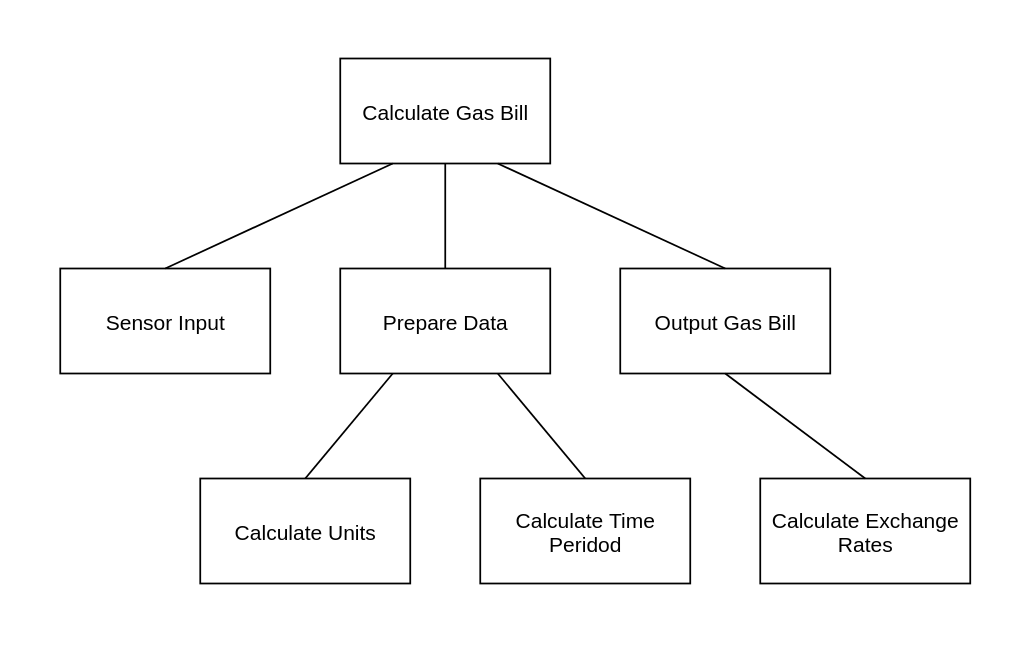
\includegraphics[width=0.9\textwidth,keepaspectratio, frame]{./images/heirarchy.png}
\caption{Example hierarchy chart}
\end{figure}

\subsection{Testing}
\label{sec:org3cd2995}

All algorithms should be thoroughly tested to detect problems that could occur under certain conditions. Any inputs should be tested with \emph{normal}, \emph{boundary} and \emph{erroneous} data. Before running a program, it may be \emph{dry-run}, using a trace table.

\subsection{Abstraction}
\label{sec:orge729003}

\emph{Abstraction} is the process of simplifying something by removing unnecessary details. This is a common technique in programming, as most high-level operations are made irrespective of the hardware and machine operations that need to take place.

Abstraction by \emph{generalisation} is a technique used to remove context from a problem and equate it to existing problems and scenarios. Therefore, the problem can be worked on in a theoretical manner and once solved, applied to the initial problem. Similar is the idea of \emph{problem abstraction}, where the problem is abstracted and generalised to a point where it matches an existing problem and solution.

\emph{Procedural abstraction} is often used in computing. Once a problem has been solved and implemented, there is no need for that module to be re-written. This is \emph{information hiding}, as the program calling a module does not need to know its implementation. This kind of abstraction depends on the existing implementation of a problem's solution.

Data can also be subject to abstraction. The behaviour of numbers, when subject to mathematical operations, depends on the number's type, eg. float or integer, rather than the program code.

\subsection{Composition}
\label{sec:org3e45b64}

Breaking an algorithm down, via any method, is called \emph{decomposition}. The process of combining existing smaller modules to solve a larger problem is called \emph{composition}.

\subsection{Automation}
\label{sec:org02ab914}

\emph{not implemented}

\subsection{Finite State Machines}
\label{sec:orgd3c9f99}

A \emph{finite state machine} is an abstract view of some computation. Using \emph{states} and \emph{transitions}, an FSM demonstrates how a system responds to an event under various conditions (states).

A state is represented with a circle. States are joined by an arrow (direction is important), representing a transition. A transition is usually labelled with a transition \emph{condition}.

The start state is marked by a short arrow, with no connection to another state. The end or \emph{acceptance} state is a double circle. See the diagram below.

\begin{figure}[H]
\centering
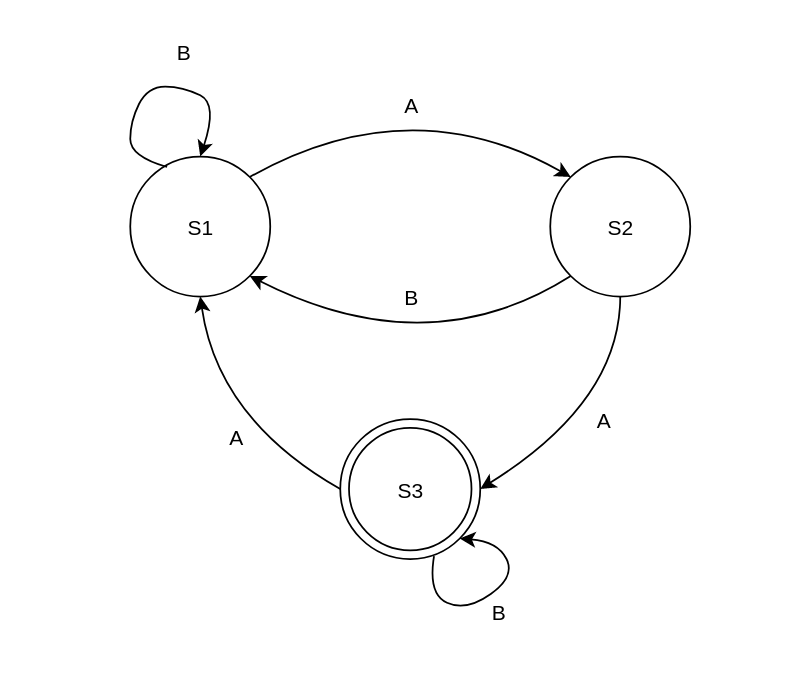
\includegraphics[width=0.9\textwidth,keepaspectratio, frame]{./images/fsm.png}
\caption{FSM with three states}
\end{figure}

The typical FSM diagram can also be represented by a \emph{state transition table}, which lists all of the possible transitions. The table for the diagram above would look like this:

\begin{center}
\begin{tabular}{lll}
\hline
current state & input = A & input = B\\
\hline
S1 & S2 & S1\\
S2 & S3 & S1\\
S3 & S1 & S3\\
\hline
\end{tabular}
\end{center}

\section{Data Representation}
\label{sec:orgd21cd64}
\subsection{Number Systems}
\label{sec:orgdc10ed6}
\subsubsection{Sets of Numbers}
\label{sec:org44a809d}

\begin{itemize}
\item Whole Numbers = \emph{Z} (negative or positive integers)
\item Natural Numbers = \emph{N} (integers above 0)
\item Rational Numbers = \emph{Q} (can be expressed precisely as a fraction)
\item Real Numbers = \emph{R} (anything that can be expressed numerically, includes irrational numbers)
\item Ordinal Numbers: \emph{first}, \emph{second}, \emph{third}
\end{itemize}

\subsubsection{Decimal}
\label{sec:org7a2c489}

Decimal (Base 10) is the number system we use on a daily basis. It may originate from the ten fingers and toes humans have. With current technology, it is impossible to use base 10 in computer systems.

\subsubsection{Binary}
\label{sec:orgc600c8f}

Binary is the number system used in computing and understood by a computer's processor. It is used because of the relative ease of distinguishing between just two states: \emph{on} \& \emph{off}. The disadvantage of this system is representing large amounts of complex data. With only two states, many binary bits in sequence are needed to represent real world data. In decimal, 10 values can be represented with one character and the total number of values available with \emph{n} characters is:

\begin{itemize}
\item \(10^{n}\)
\end{itemize}

While, with binary, the number of available values when using \emph{n} bits is:

\begin{itemize}
\item \(2^{n}\)
\end{itemize}

So in order to get an equivalent range of values, the value \emph{n} must be larger when using binary. This is manageable in a computer and the advantages significantly outweigh the disadvantages, however this is difficult for people to work with and understand. Binary is long and repetitive, making working with binary slow and error prone.

\subsubsection{Hexadecimal and Octal}
\label{sec:orgc893782}

Hexadecimal (Base 16) and Octal (Base 8) are used to make working with computers easier. The range of values that can be represented with \emph{n} place values is:

\begin{itemize}
\item \(16^{n}\) for hexadecimal
\item \(8^n\) for octal
\end{itemize}

These number systems in particular are used to represent binary values more concisely, while being easier to convert to and from binary than decimal numbers. Both 8 and 16 are powers of 2; this means that numerous individual bits of a binary number are represented by a single character or value in one of these number systems.

\begin{itemize}
\item 1 octal place value can represent exactly 3 binary bits
\item 1 hexadecimal place value can represent exactly 4 binary bits
\end{itemize}

The same is true of Base 4 and Base 32, but these are not used nearly as frequently.

\textbf{Uses of Hexadecimal or Octal number systems:}

\begin{itemize}
\item Colour Codes
\item MAC Addresses
\item IPv6 Addresses
\item Assembly Language
\item Unix File Permissions
\end{itemize}

\subsection{Two's Complement}
\label{sec:org98b909e}

There are a number of different techniques for handling negative numbers in computer systems. \emph{Two's Complement} is a common method of doing so, as two's complement numbers can be treated like a regular value during computation.

In Two's complement binary, the most significant bit of a number is treated as negative, hence:

\begin{itemize}
\item \emph{if a number begins with 1, its value will be negative}
\item \emph{if a number begins with 0, its value will be positive}
\end{itemize}

In the table below, a few examples of a 4-bit two's complement number are given. The whole number is written in the left column and is also broken down into place value columns to the right.

\begin{center}
\begin{tabular}{rrrrrr}
\hline
number & -8 & 4 & 2 & 1 & decimal value\\
\hline
1000 & 1 & 0 & 0 & 0 & -8\\
1111 & 1 & 1 & 1 & 1 & -1\\
0000 & 0 & 0 & 0 & 0 & 0\\
0101 & 0 & 1 & 0 & 1 & 5\\
1011 & 1 & 0 & 1 & 1 & -5\\
\hline
\end{tabular}
\end{center}

The decimal value in the right-hand column is the sum of all the place value columns containing a \(1\). This procedure is broken down below.

\begin{figure}[H]
\begin{minted}[ frame=single, framesep=8mm, rulecolor=RuleGray, baselinestretch=1.3, fontsize=\small, breaklines, fontfamily=tt]{text}
1111 = (-8) + 4 + 2 + 1 = -1
1000 = (-8) + 0 + 0 + 0 = -8
0000 = (-0) + 0 + 0 + 0 = 0
0101 = (-0) + 4 + 0 + 1 = 5
1011 = (-8) + 0 + 2 + 1 = -5
\end{minted}
\end{figure}


With \emph{n} bits, the range of values you can represent is:

\[2^{(n-1)}  \text{ ... } 2^{(n-1)}  - 1\]

To obtain the two's complement of a number (negative to positive or vice versa), flip all of the bits and one.

The benefit of the two's complement system is that it maximises the range of values which can be represented by a \emph{word} of a certain length, eg. using a designated sign bit a value for zero and negative zero must be stored, which is not needed and can complicate some calculations.

Computers generally rely on two's complement to perform subtraction, using only the addition circuits at their disposal. In order to subtract one value from another:

\begin{itemize}
\item the number that must be subtracted is converted to its two's complement
\item the two numbers are now added to one another
\item therefore \(37 - 9\) becomes \(37 + (-9)\)
\end{itemize}

\subsection{Fixed Point Binary Numbers}
\label{sec:orgec6a043}

In a fixed point binary value, some bits fall before and after the point. The position of the point is usually determined as needed. Using such a system, any bits before the point are treated as usual. For any bit after the point, its value is \(2^{-n}\), where \(n\) is the position from the decimal point.

Here is a demonstration of this principle:

\begin{center}
\begin{tabular}{rlr}
\hline
n & power of 2 & value\\
\hline
1 & \(2^{-1}\) & 0.5\\
2 & \(2^{-2}\) & 0.25\\
3 & \(2^{-3}\) & 0.125\\
\hline
\end{tabular}
\end{center}

The position of the decimal point within a fixed point binary value can determine the properties of the number: \emph{range} vs \emph{precision}

\subsection{Floating Point Binary Numbers}
\label{sec:org2f57923}

Fixed point binary numbers only offer limited precision, unless an extra-ordinary number of bits are used. Many bits are needed to represent very small fractions and many bits are needed to represent very large numbers, even if fixed point binary is not applied. \emph{Floating Point} binary values work like scientific notation, making them suitable for extremely large or small numbers. In such a number the bit pattern used is split into two parts: the \emph{mantissa} and the \emph{exponent}.

\subsubsection{Conversion}
\label{sec:org7151a78}

This table shows how to convert \texttt{01101 011} into a fixed point binary number. When given a floating point number, the point's default position is just after the first bit (as in scientific notation). The mantissa records how many places to the right the point needs to move. (Nb. on the first row, the default position of the point is shown)

\begin{center}
\begin{tabular}{rrr}
\hline
mantissa & exponent & exponent decimal\\
\hline
0.1101 & 011 & 3\\
01.101 & 010 & 2\\
011.01 & 001 & 1\\
0110.1 & 000 & 0\\
\hline
\end{tabular}
\end{center}

\subsection{Character Encoding}
\label{sec:orgefb7e2d}

Human readable characters need to be represented numerically for use in computer systems. The given numerical value for a character can be expressed in decimal, but binary is always used by computers. Two very common standards for character encoding are \emph{ASCII} and \emph{Unicode}. Note that not all data is encoded with these standards; compiled code and many image formats are \emph{raw binary} data. This kind of data cannot be read by a human or displayed in a text editor.

\subsubsection{ASCII}
\label{sec:org4f5679f}

The first major encoding standard was ASCII. ASCII was designed to be a 7 bit standard, allowing 128 different characters to be represented, while leaving space for a parity bit within each byte. Later on, an eighth bit was added to extend the number of possible characters which could be used. The new 8 bit ASCII maintained compatibility with the original standard; the first 128 characters are the same. 8 bit \textbf{ASCII} is sometimes called \textbf{UTF-8}.

\subsubsection{Unicode}
\label{sec:org85e5ae1}

As the internet became pervasive and computers in all parts of the world became connected, a new standard was needed to manage more languages and their character sets. \emph{Unicode} was developed to solve this problem. It was initially a 16 bit standard, allowing 65,536 different characters to be represented, enough for multiple character sets. The first 8 bits of this character set matched those of 8 bit \textbf{ASCII}, so there is some compatibility. \textbf{UTF-32} now exists, offering over a million different individual characters. The downside of these enlarged standards is the size. \textbf{UTF-32} is twice as large as \textbf{UTF-16} and twice as large again as ASCII. This means text encoded with Unicode will take up more storage on a computer and take longer to transmit.

\subsection{Error Checking and Correction}
\label{sec:org7291392}

Errors can occur when data is read, inputted or transmitted. There are many ways to identify when an error has occurred and how errors can be corrected.

\subsubsection{Parity Checking}
\label{sec:orgcd3fc73}

Parity bits are a common method for protecting against errors during communication. 7 bit \emph{ASCII} lends itself towards transmitting a parity bit within each byte. Even or odd parity may be used. The parity bit ensures that the total of all the bits (including the parity bit) is an odd or even number in accordance with the technique being used. Upon receiving data, the recipient can check the total of the bits. If the total does not correspond to the chosen parity, an error has occurred. This method cannot detect \emph{transposition errors} (when the order of bits is changed), nor are they able to identify errors affecting more than one bit.

\subsubsection{Majority Voting}
\label{sec:org175653b}

When majority voting is used, each bit is transmitted repeatedly. An odd number of repetitions must be used so there is not a \emph{tie}. The received values for each bit are compared and the \emph{popular} result is taken to be the true value of that bit. Hence, there is a means of correcting potential errors. Eg. one of three transmissions of a single bit may differ from the two others. It can be concluded that this bit is erroneous and its value discarded. Transmitting data repeatedly, for the purpose of error detection and correction, significantly increases the time taken to send a certain communication. Majority voting is often infeasible, because of the time it takes.

\subsubsection{Checksum}
\label{sec:org13ecb61}

A checksum is a thorough method of error detection. An algorithm is applied to a piece of data before it is sent, the result being the checksum. The checksum is transmitted with the block of data. Upon receipt of the block, the same algorithm is applied to the data (which might have been corrupted). The checksum calculated by the receiver is compared with the transmitted checksum. If the two values do not match, an error has occurred. If the two values do match, it is likely that no error has occurred.

\subsubsection{Check Digits}
\label{sec:orgf026f22}

The role of a \emph{check digit} is to prevent \emph{transcription} errors (or other similar I/O errors) of identifiers and other short pieces of data. Check digits are often attached to barcodes, ISBNs and credit card numbers.
A checkdigit is calculated by running a number through an algorithm. The result is usually printed alongside the data, wherever it appears. Devices like barcode readers can calculate the checkdigit based on the obtained number and compare it too the existing checkdigit. If the two values do not match, an error has occurred. If the two values do match, it is likely that no error has occurred.

\subsection{Analogue and Digital Data}
\label{sec:org498c861}

Analogue data is \emph{continuous}, having physical quantities which are changing constantly. This kind of data can only be truly represented by a continuous range of values. For the sake of digital representation, analogue waveforms and other continuous sets of data are sampled at intervals, or in certain places. Each of these samples contains data which is quantifiable, so it may be used and stored by a computer. Therefore any digital representation of analogue data is an approximation of some quantity at a certain time and place.

\subsection{Image Representation}
\label{sec:org750c1f1}

Image data can be broadly categorised into two types: \emph{photographs} and \emph{digital graphics}. While there is no scientific definition for either of these terms, a photograph is generally captured by a camera, while computerised digital graphics are typically designed or generated. Photographs are usually stored as \emph{bitmap} images, while \emph{vector} graphic files are more suitable for computerised images.

\subsubsection{Bitmap Files}
\label{sec:org639c12a}

Bitmap images are composed of \emph{pixels}. A 'picture element', or a \emph{pixel}, is the smallest identifiable area of an image and each pixel will contain information about the image at that point.

A raster (bitmap) file itself contains all of the pixel data making up the image and some \textbf{Metadata} needed to reconstruct the image. A bitmap file has a \emph{size}, which is a number of pixels expressed in terms of \emph{width * height}.

The \emph{resolution} is the number of \emph{dots per inch} (dpi). An image of greater \emph{size} will have a higher \emph{resolution} when displayed in the same space/scale on a screen.

Bitmap files store an approximation of real world analogue data and they are ideal for photographs, which have constantly changing colour gradients and no distinct boundaries.

\subsubsection{Limitations of Bitmap Files}
\label{sec:orga52c603}

The \emph{size} of an image (in pixels) does not determine the area its is displayed on. Should an image need to be displayed in a physical form that is greater than the original dimensions, the resolution (ppi/dpi) is diminished. For simple graphics, a bitmap file's size may exceed that of a vectorised file format.

\subsubsection{Colour Depth}
\label{sec:orgfdd7847}

In a bitmap file, each picture element has an associated colour code. The length of this value determines the number of colours which can be represented.

A common colour depth is 3 bytes (24 bits), where each byte corresponds to one \emph{RGB} channel. Each channel has 8 bits and so the number of possible colours (in each channel) is:

\emph{2\textsuperscript{8} = 256}

As there are three channels, the total number of colours is:

\emph{256\textsuperscript{3} = 16777216}

A colour depth of 3 bytes offers more colours than the human eye can distinguish between, hence there is little benefit using a greater depth. A larger colour depth increases file size, so it is sometimes advantageous to use a reduced set of colours.

\subsubsection{Metadata}
\label{sec:org0ea344c}

This is data stored in the header of a bitmap file, containing all the information needed to display the image. Eg. columns, rows, colour depth, etc.

\subsubsection{Vector Graphics}
\label{sec:org5150539}

A vector file consists of a drawing list, containing a list of all the shapes that need to be drawn to \emph{construct} the image. Unlike a bitmap, the shapes listed in a vector file can be redrawn and the image constructed proportionally to suit any display size. This makes vector graphics ideal for images which may need to be displayed in many places at different sizes.

The file size of a vector graphic will depend on the number of objects which have to be drawn, rather than the size and quality of the image. Photographs cannot be represented with vector graphic files easily, because of the complex shapes and many colour gradient, with few distinct boundaries.

\subsection{Audio Representation}
\label{sec:org7e868c2}

Sound is a type of analogue data, which is - in nature - a continuous wave. This data must undergo analogue to digital conversion.

\subsubsection{Sample Rate}
\label{sec:orgac5b931}

In order to represent a continuous sound wave as discrete digital data, many quantised \emph{samples} must be taken at regular intervals. The frequency of the recording, also called the \emph{sample rate}, is the number of samples per second. The greater the sample rate, the closer the digital representation of the audio is to the original sound.

\subsubsection{Sample Depth}
\label{sec:orgb882deb}

As well as increasing the number of samples stored, audio quality can be improved by increasing the \emph{bit depth}. The bit depth is the number of bits used to store the amplitude of the sound at a given sample. The higher the bit depth, the closer the amplitude to its original value. \emph{Nb. amplitude is often represented on the Y axis, against time on the X axis}

\subsubsection{Nyquist's Theorem}
\label{sec:org7cb15a1}

Discrete digital data cannot perfectly represent all of the properties of a continuous analogue waveform. In 1928, Harry Nyquist theorised that a recording must be sampled at twice the maximum frequency of the analogue sound to produce an accurate recording. For the human ear, the maximum audible frequency is 20,000Hz. Therefore, audio is often sampled at 44,100Hz, beyond which there is no apparent difference in sound quality to humans.

\subsubsection{Audio Storage and Files}
\label{sec:orgb9d4c74}

Audio which is recorded from a live source is stored and can be played back using a DAC and a speaker. There are many common file formats for sound and video, many of which use compression. Sound files may also contain metadata about the file.

Sound may also be 'stored' as a MIDI file, a set of steps which can be interpreted by software to synthesise new sound. It is primarily a tool for music artists to create new music which can later be recorded. As MIDI files do not try to replicate analogue data with lots of samples, they may be smaller in size to a recording of similar length and quality.

\subsubsection{Recording}
\label{sec:org25141ec}

\begin{enumerate}
\item A computer peripheral (microphone) is used to convert a sound wave into an oscillating electrical signal.
\item The electrical signal is suitable for analogue to digital conversion.
\item An ADC will \emph{sample} this signal to a given frequency. Any data between samples is lost.
\item The ADC will approximate the amplitude of the sound for each sample.
\item The output - discrete digital data - can be stored in typical computer storage devices.
\end{enumerate}

\subsubsection{Playback}
\label{sec:orgb23afaa}

\begin{enumerate}
\item In order to present the stored data, it must be converted back to an analogue form. A \emph{DAC} (digital to analogue converter) can be used to this effect.
\item The recorded amplitudes for all the samples are converted into an electrical signal (a voltage) at the same frequency as the sample rate.
\item The voltage changes are converted into a sound wave by a speaker.
\end{enumerate}

\subsection{Compression}
\label{sec:org8ca81e5}

Image and sound files can be very large and repetitive. Generally, a small reduction in quality is tolerated, making these files good candidates for lossy compression, where the quality is somewhat reduced to achieve greater compression ratios.

Text files, including programs, are rarely as large as other types of data, however reducing their file size is sometimes needed. It is essential that compressed text files can be recreated without any loss in quality. Lossless compression is a compression method which maintains the exact quality of the uncompressed data, so it can be read exactly as intended after compression and subsequent uncompression. The compression ratios of Lossless compression techniques rarely equal those of lossy compression.

\subsubsection{Lossless}
\label{sec:org46fd253}

Lossless compression ensures the original file can be recreated from the compressed file. Therefore the compressed file must convey \emph{exactly} the same information as the original in a slightly different way. Lossless compression algorithms typically reduce repetition within files as a means of compression.

Most Lossless compression methods are only effective when there is significant repetition. In some cases, when there is not sufficient repetition, negative compression can occur and the size of the compressed file exceeds that of the original file.

\textbf{Run Length Encoding:}

Using RLE, file size is reduce by removing runs of identical data. Each run of data is replaced with the original piece data and the length of the run (number of repetitions).

Data which does not have long runs of identical data is not suitable for this type of compression. RLE can be very useful in the compression of sound files, as a single sound played for even a short amount of time may result in many identical samples.

\textbf{Dictionary Compression:}

Dictionary compression is a more flexible type of lossless compression. The compression algorithm creates a \emph{dictionary} associating frequently repeated pieces of data to an index. Any occurrence of an indexed piece of data are replaced with the corresponding dictionary index.

Nb. The compressed file must include the dictionary that is used. Dictionary compression works best with larger files, where the size of the dictionary is offset by the amount of repetition removed.

\subsubsection{Lossy}
\label{sec:org0d9eb72}

Unlike lossless compression, lossy compression is irreversible, as data is \textbf{permanently} removed from the file. This means that the effectiveness of lossy compression is not dependent on an amount of repetition within the file. However, this method reduces the quality of the file which is compressed, making it unsuitable for text and similar sorts of data.

\subsection{Encryption}
\label{sec:org6d7ae9f}

Encryption is the process of changing data so that it is only readable to the intended recipient. A cipher is an algorithm which encrypts some data. Decryption of cipher text requires the \emph{key} used to encrypt the file and the encryption method must be known. The original data is referred to as plain text and the encrypted data is referred to as cipher text.

\subsubsection{Caesar Ciphers}
\label{sec:org2fe4cad}

This is a very old, basic cipher, using character replacement. One character in the cipher text always represents the same plain text character.

A shift can be used to quickly generate a cipher. The ciphertext value of a character is found by moving a certain number of places through the alphabet. In this case, the key is the shift required to move from the plain-text to the ciphertext. This process can be reversed by the recipient to decrypt the data.

A substitution cipher may also be used. With such a cipher, the letters are randomly replaced. This introduces more complexity as there is not a single key that applies to the whole data. To decrypt such a cipher the 'key' for each character must be known to the recipient.

All Caesar ciphers are fairly easy to decipher without the key. In the case of a shift cipher, brute force is possible as there are only 25 possible keys. Frequency of the ciphertext characters can be analysed as every occurrence will refer to a certain plain text character. In English, certain characters and combinations are more frequent so the most common cipher text characters can be found and decrypted.

\subsubsection{Vernam Ciphers}
\label{sec:org8dbe7f3}

The Vernam cipher is a more secure algorithm. It requires a key in the form of a one-time pad. \emph{One-time} means it should only be used once, to ensure its randomness. The key must be as long, or greater than, the plain text to be encrypted.

\textbf{Encryption:}

\begin{itemize}
\item Plain text is aligned with the beginning of the one-time pad
\item The characters are represented numerically, in binary
\item A logical XOR process is performed on the plain text and one-time pad bit patterns
\item The resulting bit pattern is translated back into a character
\end{itemize}

\textbf{Decryption:}

\begin{itemize}
\item To decrypt the cipher text, the same one-time pad must be used
\item The two strings are aligned
\item Both strings are converted to binary
\item The logical XOR operation is carried out
\item The resulting bit pattern is converted back to a character, which should equal the initial plain text character
\end{itemize}

The one-time pad which is used must be generated randomly, only this can guarantee the randomness of the ciphertext. If the pad is new and random, the ciphertext is completely unbreakable at the point it is encrypted. This cipher is mathematically unbreakable, if all standards are upheld. To make this cipher more efficient, an amount of pad may be exchanged between parties before any messages are sent. Each message sent will use the next unused section of pad as the key.

Vernam ciphers are not always used in computer systems, even though it is mathematically secure. Given current computing power, many other algorithms - which can be cracked - will take long enough that any efforts to crack the encryption will not be viable. This is called computational security.

\section{Hardware and Software}
\label{sec:org09bb612}

Hardware is the name given to physical equipment that constitutes a computer. Meanwhile, software is program code stored digitally and used to perform a task.

\subsection{Classification of Software}
\label{sec:org52a4833}
\subsubsection{System Software}
\label{sec:org70841a3}

System software is the collection of software needed to run a computer system, including an operating system. A general purpose operating system will usually ship with additional software to make the computer more functional. There are other types of system software.

\begin{enumerate}
\item Operating Systems
\label{sec:orgb1a9f12}

An operating system \emph{(OS)} is a piece of software designed to manage a computer's hardware on behalf of running applications and ultimately the computer user. The operating system interacts directly with the system's resources, exposing available operations to other applications, a good example of a programming \emph{API}. The benefit of an operating system is versatility. With an \emph{OS} installed there is no need for each application to perform low level operations and the computer will be able to perform many different tasks without reprogramming.

\textbf{Common OS tasks:}

\begin{itemize}
\item multi-processing and multitasking
\item backing store management
\item device and driver management
\item hardware diagnostics
\item detecting peripherals
\item interrupt handling
\end{itemize}

\item Utility Software
\label{sec:orgee78507}

Utility software is often included with an operating system to help maintain the machine, but the user may choose to install more of these utilities. Typically, the operating system itself will use the installed utility software, although the user may choose to use the software manually.

\textbf{Examples include:}

\begin{itemize}
\item disk management
\item virus checking
\item file management
\item compression tools
\item software installer/uninstaller
\end{itemize}

\item Code Libraries
\label{sec:org5dd3dd4}

Many programming languages have a library of code that is \emph{built-in}, to simplify common operations. This code can be packaged and implemented in many different ways, but the core functions are usually included with the language and stored on a users computer. Some common library extensions are: \textbf{.dll} and \textbf{.so}. Should a program need functionality from the libraries, it is \emph{imported} in the source code.

\item Translators
\label{sec:org2b7c235}

Translators are required to transform written source code into executable machine code, with various steps along the way. The different types of translators are covered below.
\end{enumerate}

\subsubsection{Application Software}
\label{sec:orgd568491}

Application software is designed to work on a certain operating system and perform tasks for the user. This type of software may be shipped along with an operating system, although a user may choose to install or remove this type of software on a regular basis. Application software is developed in different ways for different customers. Here are some common ways software is made and distributed: \emph{General Purpose}, \emph{Specific Purpose} and \emph{Bespoke}.

\begin{enumerate}
\item General Purpose
\label{sec:orga92eac2}

\begin{itemize}
\item Includes mainstream products like office suites or graphics programs
\item A user will install this kind of software to help with whatever specific purpose they have in mind
\item This type of software will be used by many people to achieve different results
\end{itemize}

\item Special Purpose
\label{sec:org9729a58}

\begin{itemize}
\item This is also a type of application software, but unlike general purpose software, this type of software serves a more specific audience
\item This type of software is still widely available and its specificity does not reduce its pervasiveness
\item E.g. a python IDE is specific software, but many people will use this software.
\item This type of software does not necessarily match the exact requirements of a person or business, as this type of software is published without a specific customer in mind and it may be disseminated to many people
\end{itemize}

\item Bespoke Software
\label{sec:orge7c1d48}

A business may choose to have software developed specially for them by some software developers. This is called \emph{bespoke software}.

\begin{itemize}
\item This kind of software is generally special purpose, as there is no need to create new general purpose software
\item Bespoke software means it not only serves a specific purpose, it is also created directly for a specific customer
\item The benefits of a bespoke system is ease of use and specificity (no redundant/missing features, because the client told the developer what to include)
\item The downside of this type of software is the time and cost associated with developing the software after the need is identified
\item Additionally, the software may not be stable if it has not been tested extensively by others
\end{itemize}
\end{enumerate}

\subsection{Programming Language Specification}
\label{sec:org71d3743}
\subsubsection{Low-Level Languages}
\label{sec:org96704bd}

The two main types of low-level language are \emph{machine code} and \emph{assembly language}.

\begin{enumerate}
\item Machine Code
\label{sec:orgfbea816}

Machine code is written entirely in binary and as a result it can be executed by a computer without the need for translation. At this level, abstraction is limited and a program consists of the set of operations the processor must perform.

Machine code instructions are composed of an \emph{opcode} and associated \emph{operands}. The available opcodes depend on the processor's \emph{instruction set} and so machine code is specific to the platform it was designed for, therefore machine code is not \emph{portable}.

Binary is repetitive and lengthy, making mistakes like transcription errors very common. Once a program has been developed, the machine code is difficult to understand and debug.

\item Assembly language
\label{sec:org2a309c4}

Assembly language was designed to make working with native machine code easier. Opcodes are replaced by mnemonics, while hexadecimal and decimal numbers are often used in place of operands. Assembly language reduces the amount of errors made when inputting code and makes the code easier to read and understand.

Generally speaking, each line of code in an assembly language program corresponds to a single machine code instruction; the extent of assembly language abstraction is limited. This means that assembly language is processor specific, like machine code. In addition, assembly code shares the same detailed approach to programming, as each line of code is a single processor instruction, rather than part of an algorithm.
\end{enumerate}

\subsubsection{High-Level Languages}
\label{sec:orga1b290a}

As \emph{operating systems} developed, it became possible to write programs which could be run on many platforms.  The languages used to write these programs became known as \emph{high-level} languages. A high-level language will need to be converted, or \emph{translated}, into executable code for each platform it is used on.

High-level languages are much easier to read, write and understand, thanks to the \emph{abstraction} of factors like computer hardware and system resources. Code written in a high-level language more closely models spoken language and uses common symbols like \texttt{+} and \texttt{-}, along with named variables, comments and indentation to improve ease of use.

High-level languages are much more suitable for designing complex algorithms, as each line describes a single step in the problem, rather than the processor operations needed to make it happen.

A programming \emph{paradigm} is a way of classifying high-level programming languages. The \emph{Imperative} programming language paradigm includes both the \emph{procedural} and \emph{object orientated} techniques. Meanwhile, the \emph{declarative} paradigm includes languages like SQL and the \emph{functional} programming style.

\subsubsection{Abstraction}
\label{sec:org1f28676}

High-level languages are more \emph{abstract} than low-level languages. Each line of python contains far more operations than a line of x86 assembly. Should a process need to be made very efficient, the very minimum level of abstraction should be used. If some process involves specific hardware, it may be useful to use a low-level language to get the best performance from it.

\subsection{Programming Language Translation}
\label{sec:orge547c94}

Besides native machine code, all other types of programming language, including assembly, need to be converted into a format the computer can understand. This process is called \emph{translation}. The two most common methods of translating source code written in a high-level language into object code are \emph{compilation} and \emph{interpretation}.

\subsubsection{Assemblers}
\label{sec:orge83e662}

While assembly is a type of low-level language, it requires translation. The tool used to do this is called an \emph{assembler}. The result of running assembly code through an assembler is object code. Object code may need to be run through a \emph{linker} program to make executable code (not on specification).

\subsubsection{Compilers}
\label{sec:org9e60f61}

A compiler is a program that can translate code written in a high-level language into executable code. The compiler program runs over inputted source code, performing a series of checks and identifying how to construct the object code output.

A program written in a compiled language is usually distributed by sharing the compiled object code, which can be run in the absence of the compiler. This means the original code can be kept private or \emph{closed source}.

\textbf{Advantages of a Compiler:}

\begin{itemize}
\item Errors are detected before translation
\item Compiled code can be run without the need for translation, making execution faster
\item Compiled code can be distributed without compromising the source code
\end{itemize}

\subsubsection{Interpreters}
\label{sec:orge5a2de1}

An interpreter translates a program into executable machine code instructions at run-time. Sometimes there is an intermediate type of compiled code, called \emph{bytecode}.

A typical interpreter will scan source code in advance for syntax errors, and subsequently translation happens line-by-line. The interpreter will call subroutines within its own source code to handle high-level instructions in the input code.

As the interpreter works line by line, some code may be translated and run before an error is reached.

\textbf{Advantages of an Interpreter:}

\begin{itemize}
\item No long periods of compilation
\item Identifying errors and debugging the program is easier
\end{itemize}

\subsubsection{Bytecode}
\label{sec:org834a17b}

In order to improve the performance and portability of high-level code, \emph{bytecode compilation} is sometimes used (usually in interpreted languages). This divides the compilation process into two parts:

\begin{enumerate}
\item \emph{bytecode compilation}
\item \emph{machine code translation}
\end{enumerate}

Implementations of this process vary. Some languages like \textbf{java} have a portable \emph{virtual machine}, capable of interpreting bytecode. Once source code has been compiled into bytecode for the java virtual machine, it can be run anywhere the \emph{JVM} is installed.

In the case of java, bytecode for the \emph{JVM} is distributable. With the standard python implementation, the bytecode compiler and the interpreter are not separable; bytecode compilation and translation happen at run time. As a result the source code must be shared to distribute the program. It is possible to present python bytecode in human readable form. Here is a program that demonstrates this:

\begin{figure}[H]
\begin{minted}[ frame=single, framesep=8mm, rulecolor=RuleGray, baselinestretch=1.3, fontsize=\small, breaklines, fontfamily=tt]{python}
import dis

def hello():
    print("hello")

hello()
dis.dis(hello)
\end{minted}
\end{figure}

The output of the script is as follows:

\begin{figure}[H]
\begin{minted}[ frame=single, framesep=8mm, rulecolor=RuleGray, baselinestretch=1.3, fontsize=\small, breaklines, fontfamily=tt]{text}
hello
  7           0 LOAD_GLOBAL              0 (print)
              2 LOAD_CONST               1 ('hello')
              4 CALL_FUNCTION            1
              6 POP_TOP
              8 LOAD_CONST               0 (None)
             10 RETURN_VALUE
\end{minted}
\end{figure}

\subsection{Boolean Logic \& Algebra}
\label{sec:org7205496}

\subsubsection{De Morgan's Laws}
\label{sec:org62eeb83}

\[\overline{A + B} = \overline{A}  \boldsymbol{\cdot} \overline{B}\]

\[\overline{A \boldsymbol{\cdot} B} = \overline{A} + \overline{B}\]

\subsubsection{General Rules}
\label{sec:orge3586f4}

\[X \boldsymbol{\cdot} 0 = 0\]

\[X \boldsymbol{\cdot} 1 = X\]

\[X \boldsymbol{\cdot} X = X\]

\[X \boldsymbol{\cdot} \overline{X} = 0\]

\[X + 0 = X\]

\[X + 1 = 1\]

\[X + X = X\]

\[X + \overline{X} = 1\]

\[\overline{\overline{X}} = X\]

\subsubsection{Commutative Rules}
\label{sec:org55920ed}

\[X \boldsymbol{\cdot} Y = Y \boldsymbol{\cdot} X\]

\[X + Y = Y + X\]

\subsubsection{Associative Rules}
\label{sec:orga61f065}

\[X \boldsymbol{\cdot} ( Y \boldsymbol{\cdot} Z) = ( X \boldsymbol{\cdot} Y) \boldsymbol{\cdot} Z\]

\subsubsection{Distributive Rules}
\label{sec:org78a21a9}

\[X \boldsymbol{\cdot} (Y + Z) = X \boldsymbol{\cdot} Y + X \boldsymbol{\cdot} Z\]

\[(X + Y) \boldsymbol{\cdot} (Z + W) = X \boldsymbol{\cdot} W + X \boldsymbol{\cdot} Z + Y \boldsymbol{\cdot} Z + Y \boldsymbol{\cdot} Z\]

\subsubsection{Absorption Rules}
\label{sec:org3c4326f}

\[X + (X \boldsymbol{\cdot} Y) = X\]

\[X \boldsymbol{\cdot} (X + Y) = X\]

\section{Computer Organisation and Architecture}
\label{sec:org48e7758}
\subsection{Harvard \& Von Neuman Architecture}
\label{sec:orgfd8a3a0}

Many early computers could only perform one operation. The \emph{Stored Program Concept} allows a computer to store its instructions in re-programmable memory. This means that a computer could be instructed to perform a new operation without the disassembly of the machine. There are two main types of computer architecture designed with this general purpose computing paradigm in mind.

The \emph{Harvard} architecture separates instructions and data, having a dedicated area of memory for each. The advantage of this setup is the computer's ability to fetch data and instructions simultaneously. In addition, a processor with this architecture can have a custom memory configuration depending on its purpose. This architecture is common among embedded systems.

The \emph{Von Neuman} architecture has only one area of memory for both instructions and data. Instructions and data have to be fetched serially, which is often slower. However, this architecture is much more flexible and is used in most general purpose personal computers and mobile devices.

\subsection{Motherboard}
\label{sec:orga3b5d26}

A Computer's motherboard connects all the components of a computer together. The Central Processing Unit (\emph{CPU)} is housed on the motherboard. The motherboard also houses the computer's interfaces to external components, including the \emph{RAM} and \emph{IO} devices. Processor buses join components on the motherboard, allowing the \emph{CPU} to control the operation of the whole computer.

\subsection{CPU Disambiguation}
\label{sec:org9316908}

\emph{CPUs} are implemented on a Integrated Circuit \emph{IC} metal-oxide-semiconductor \emph{MOS} microprocessor chip. Many chips have more than one processor core, these chips are called \emph{multi-core processors}. Each core may have more than 1 thread, creating \emph{virtual cores}. A chip with multiple cores, virtual or physical, will appear to the operating system as multiple \textbf{CPUs}. The A-Level specification describes the operation of a single \emph{CPU}.

In short, a \emph{processor} is mounted on a \emph{motherboard} and may have multiple \emph{CPUs}, whether they be physical cores or virtual threads.

Silicon is a useful material for constructing processors. Silicon has semiconductor properties which mean it can behave like a switch, becoming conductive under certain conditions. The flow of charge is how processing works and so changing the conductivity of the chip is required.

\subsection{CPU Components}
\label{sec:org517cf71}
\subsubsection{Processor Clock}
\label{sec:org2804b68}

The system clock generates an oscillating signal, with a frequency in the billions of Hz range. One clock cycle is the time taken for the clock to return to its default position. A CPU operation begins at the beginning of a clock cycle and cannot be complete until the clock cycle has finished. One CPU operation may span many clock cycles.

\subsubsection{Control Unit}
\label{sec:orgd692c37}

All the operations and flow of data around the CPU is governed by the control unit. Once an instruction is received, the control unit will organise its execution, including any required mathematical operations in the \emph{ALU}. The control unit also handles data operations, including accessing main memory and general purpose registers.

\subsubsection{Arithmetic and Logic Unit}
\label{sec:orgd40250d}

The \emph{ALU} contains circuits capable of most mathematical operations and services requests from the control unit. The ALU will store some information as flags in the \emph{Status Register}, important when making comparison operations.

\subsubsection{General Purpose Registers}
\label{sec:org417b11f}

Modern computer processors have 16 general purpose registers. These are areas of fast, expensive, on-chip storage. In a 64 bit machine, one of these registers is 64 bits in size, although smaller registers are addressable, taking up the least significant bits of their larger counterparts. The data used in \emph{ALU} operations is read from and stored back into these registers.

\subsubsection{Dedicated Registers}
\label{sec:org3b9f4eb}

There are a number of specialised registers within the control unit, necessary for the operation of the computer. Unlike general purpose registers, they are not used to hold the operands and results of ALU operations.

\begin{enumerate}
\item Status Register
\label{sec:org79319af}

Following an ALU operation, \emph{flags} (individual bits) are set in the status register. These Indicate the result of the last operation. Here are some common status register flags:

\begin{center}
\begin{tabular}{ll}
\hline
symbol & purpose\\
\hline
CF & carry bit\\
PF & parity bit\\
ZF & zero\\
SF & sign bit\\
OF & overflow\\
AF & adjust\\
IF & interrupt enabled\\
\hline
\end{tabular}
\end{center}

\item Memory Buffer Register
\label{sec:org13a3e36}

Data that has been copied from main memory is stored here while it awaits an operation. Newly fetched instructions will he copied here initially before they are copied into the \emph{CIR} and decoded.

\item Current Instruction Register
\label{sec:org634ad34}

After an instruction is put in the \emph{MBR}, it is copied into the \emph{CIR} and decoded ahead of execution.

\item Program Counter
\label{sec:org6d78a85}

The program counter is responsible for managing the flow of execution. During a fetch, the value of the program counter is copied to the \emph{MAR} so that the next instruction can be retrieved. During instruction execution, the program counter is able to record the address of the next instruction so that program flow can resume after data is fetched form memory, altering the value in the \emph{MAR}. In normal operation the \emph{PC} is incremented so that the next instruction is fetched from the next address in memory, although the contents of the \emph{PC} can be modified to perform a jump and resume operation from elsewhere in the program.

\item Memory Address Register
\label{sec:org852f4a7}

The memory address register will hold an address from which data is to be retrieved or written to. Instructions are also fetched from the address held by this register during the \emph{FDE} cycle.
\end{enumerate}

\subsection{Motherboard Buses}
\label{sec:org53008a0}

The \emph{processor} is connected to other motherboard components by \emph{buses}. A bus is a \emph{parallel} wire, through which addresses, data and control signals can flow. Motherboard communication is \emph{synchronous} and the distances involved are short. There are three main buses on any motherboard, which are collectively referred to as the \emph{system bus}.

\subsubsection{Address Bus}
\label{sec:org3cc1465}

The address bus is a uni-directional wire, capable of transferring an address from the \emph{MAR} to main memory. The address bus is also used to identify \emph{IO} devices during data input and output.

\subsubsection{Data Bus}
\label{sec:org5d5db4b}

This bus is bi-directional and allows data to flow between the processor and main memory in either direction. The bus is also used to share data amongst all the other components between these two.

\subsubsection{Control Bus}
\label{sec:org52d7523}

Control signals are sent between motherboard components along this bus. The control bus is bi-directional, meaning these signals can flow either way. Here are some example control signals:

\begin{itemize}
\item memory write
\item memory read
\item interrupt request
\item bus request
\item bus grant
\item clock signals
\item reset
\end{itemize}

Many of these signals may be raised by devices other than the control unit.

\subsection{IO Controllers}
\label{sec:org12715a8}

An \emph{IO} controller sits between the processor and a peripheral device. Device controllers are addressable by the processor and receive instructions and data through the \emph{system bus}. The controller is responsible for converting \emph{CPU} input/output requests to device specific instructions during normal operation.

An \emph{IO} controller is also responsible for detecting and managing connected devices, raising processor \emph{interrupts} when action needs to be taken. This means that the processor can dedicate its time to \emph{FDE} operations rather than device management, significantly improving efficiency.

\subsection{Cache}
\label{sec:org928e250}

Cache is a small, expensive area of a computer's memory. Cache memory is sometimes located on-chip or at least very nearby. Different \emph{CPUs} will have different cache configurations. In a multi-core processor some of the cache may be shared by all of the processor cores.

A computer will often have different levels of cache, for example:

\begin{itemize}
\item L1 cache, with a size between 2 and 64 KB
\item L2 cache, with a size between 256 KB and 2 MB
\end{itemize}

\subsection{FDE Cycle}
\label{sec:orgcabc523}

Execution of a machine code instruction can be separated into three distinct phases: \emph{fetch}, \emph{decode} and \emph{execute}. In a modern computer this happens many times per second.

\subsubsection{Fetch}
\label{sec:org6a98a70}

The value of the \emph{PC} is copied to the \emph{MAR}. This address is sent to the device's memory along the \emph{address bus}. The value stored in the specified address is returned to the processor on the \emph{data bus}. This value is temporarily stored in the \emph{MBR} while the \emph{PC} is incremented and operation is synchronised with the system clock. The fetch ends as the contents of the \emph{MBR} are copied to the \emph{CIR}.

\subsubsection{Decode}
\label{sec:org129ed5c}

The machine code instruction in the \emph{CIR} is interpreted. The instruction is split into opcode and operand sections. Depending on the addressing mode (which is part of the opcode) and the requested operation, any additional data that is required is fetched and stored in one of the general purpose registers.

\subsubsection{Execute}
\label{sec:org455b3de}

The specified operation is performed, having been decoded and identified. If the \emph{ALU} is involved, \emph{status register} flags are set and the results of the operation are stored in either the \emph{accumulator}, general purpose registers or main memory, depending on the device.

\subsection{Interrupts}
\label{sec:org6a8d8f4}

During the \emph{FDE} cycle, the processor will periodically check for \emph{interrupts}. Interrupt signals are carried to the processor via the \emph{control bus}. These signals may originate from \emph{IO} controllers and hence from hardware devices, or they might be raised by running software.

When an interrupt is received and detected, the operating system determines its urgency and how to safely suspend operation and service it. When it is safe to do so, presently executing instructions and their data are pushed on to the \emph{system stack} and processor time is given to the \emph{Interrupt Service Routine}. Once the interrupt is dealt with, control returns to the processor's previous task, provided that the situation was recoverable.

\subsection{Processor Performance}
\label{sec:org6666d4d}

A number of factors affect the time a computer will take to perform a given operation or set of operations. No measure alone is able to definitively determine the performance of a computer.

\subsubsection{Clock Frequency}
\label{sec:orgd22567c}

The clock speed of a processor governs all \emph{CPU} operations, so theoretically a processor with a higher clock frequency can perform processor actions faster. In practice this is not a reliable single measurement of performance, as other factors dictate the amount of processing that can be performed with a certain number of cycles.

\subsubsection{Word Length}
\label{sec:org7d0dab4}

The word length of a processor is the number of bits that a \emph{CPU} can operate on in a single action. This value tends to be the same as the size of the processor's registers and the width of the computer's data bus. Modern, general-purpose computers tend to use a 64-bit word length. A processor with a smaller word length will have to make successive fetch operations to work on a similar amount of data to a computer with a larger word length. This will increase the number of clock cycles used to process an amount of data.

\subsubsection{Address Size}
\label{sec:org2cdbc4f}

The size of the address register and the width of the address bus limit the number of addressable memory locations in one operation. With \emph{n} bits the number of memory locations available is equal to \(2^{n}\). With 32 bits this is 4GB of memory. If there is a smaller amount of main memory, the processor will have to copy data back and forth between secondary storage and memory more frequently, to make sure that running processes are performant enough. Multi-tasking may be more difficult with less \emph{RAM}. Under certain conditions this will not affect performance at all. Nb. the length of an address is usually the same as the word length.

\subsubsection{Multiple Cores}
\label{sec:org607e17d}

A processor may have multiple CPUs, whether they be physical \emph{cores} or virtual \emph{threads}. Each CPU can perform a separate \emph{FDE} cycle, significantly improving theoretical processing capability, although not all software will be able to make use of these extra CPUs, limiting the performance gains in most situations.

\subsection{Instruction Sets}
\label{sec:org87a5889}

Computers have different ways of representing available operations to programmers. An instruction set describes the operations a processor can perform with a binary value. An instruction set is specific to a certain processor architecture. The operations that a processor can perform may be similar to those of another processor, although the instruction set, used to trigger those operations, may be entirely different. The instruction set determines how machine code is interpreted and hence written. Each instruction in the instruction set has a binary value, so machine code, which is written in binary, can be directly understood by the processor without translation.

\textbf{Typical Operations:}

\begin{itemize}
\item Data transfer
\item Arithmetic calculations
\item Comparison
\item Logical operations
\item Branch (conditional)
\item Shift (multiplication)
\end{itemize}

A machine code \emph{instruction} usually has two parts: the \emph{opcode} and the \emph{operand(s)}. The opcode corresponds to an instruction and the operand(s) are effectively arguments.

\subsection{Addressing Modes}
\label{sec:org97b688d}

When constructing a machine code instruction, part of the opcode is the \emph{addressing mode}. This defines how the arguments ought to be interpreted. There are two main types of addressing mode: \emph{immediate} and \emph{direct}.

\begin{itemize}
\item when immediate addressing is used, the value to be used in an operation is specified in the machine code instruction as a constant
\item in direct addressing, the value to perform an operation on is stored in the address given by the arguments (memory or register)
\end{itemize}

\subsection{Assembly Language}
\label{sec:org3f854a3}

Here are my x86\_64 assembly notes and examples: \url{https://github.com/alexander-neville/assembly}. AQA has its own instruction set, found here: \url{https://filestore.aqa.org.uk/resources/computing/AQA-75162-75172-ALI.PDF} and there is a simulator capable of running these instructions here: \url{https://peterhigginson.co.uk/AQA/}

\subsubsection{Fibonacci Example}
\label{sec:org7311bd3}

This is a good example of some AQA assembly. The program prints the first 10 Fibonacci numbers, using some basic operations and comparisons.

\begin{verbatim}
// initialise some variables

    MOV R0, #1 // current number
    MOV R1, #0 // previous number
    MOV R3, #0 // counter

LOOP:

    MOV R4, R0 // backup current number
    ADD R0, R0, R1 // find next number
    MOV R1, R4 // store previous number
    OUT R0, 4 // print current number
    ADD R3, R3, #1 //increment by 1
    CMP R3, #10
    BLT LOOP // repeat if not the 10th iteration
    HALT // end of program

\end{verbatim}

\subsubsection{Bit-wise Operations}
\label{sec:org207efa1}

A bitwise operation operates on each bit, irrespective of its value. To determine whether a binary number is odd or even a bitwise and operation can be used. The binary number undergoes \emph{AND} with \emph{000\ldots{}1}. This operation is shown bellow (a \texttt{-} means any value)

\begin{verbatim}

-------1
00000001
=
00000001 = 1


-------0
00000001
=
00000000 = 0

\end{verbatim}

The result is only \emph{1} if the last bit of the number is \emph{1}. Other digits are always \emph{0} after this operation. (anything and \emph{0} is \emph{0})

To flip all the bits, a logical \emph{NOT} operation can be used. Additionally a register can undergo an \emph{XOR} operation with \emph{111\ldots{}1} to achieve the same result. Once a number has been inverted, 1 can be added to find the two's complement of the original number.

\subsubsection{Logical Shifts}
\label{sec:orgabbc206}

During a shift operation, the entire contents of the register can be moved. In a left shift \emph{(LSL)}, the \emph{most significant bit} is moved out of the register. In a right shift (\emph{LSR)}, the \emph{least significant bit} is moved out of the register. The bit which is lost from the register is stored in the \emph{carry flag} in the \emph{status register}. This kind of operation can be used to check whether a number is even or odd:

\begin{verbatim}

01011011
00101101 ;; carry 1
01011010 ;; the lsb has been zeroed

01011010
00101101 ;; carry 0
01011010 ;; the result is the same

\end{verbatim}

Following a \emph{LSR} and then a \emph{LSL} the least significant bit is set to zero, irrespective of its initial zero. The result of this operation can be compared to the initial value. If the two values are not equal, the \emph{LSB} must have been a one and hence the initial value was odd.

\subsection{IO Devices}
\label{sec:orgb34d06e}
\subsubsection{Barcodes}
\label{sec:orgd129bde}

A barcode is a reliable way of storing a small amount of information. This makes them suitable for storing some sort of identification number that can be looked up in a database. It is up to retailers to store information about the associated product. Eg. Two retailers may sell the same product, with the same barcode, although each retailer will store different data about that product, including price, etc.

Many different standards are used for encoding data in barcodes. The most common are the European Article Number \emph{(EAN)}, sometimes called \emph{IAN}, and other barcode standards recognised by \emph{GS1}, a not-for-profit standards agency based in Belgium. Another common type is \emph{code 128}, which can store characters and is often used in shipping and logistics. It is the standard of the barcode that determines its appearance and how it can store data.

\textbf{Description:}

A barcode can be described as \emph{one dimensional}. The benefit of such a tall barcode with all the data arranged lengthways is reliability; the barcode can be accurately read even if part of the total height is damaged.

A barcode will typically include a \emph{quiet area} before the barcode to reduce interference. In addition \emph{guide bars} are found at the beginning, in the middle and at the end of the barcode \emph{(EAN)}. This helps frame the barcode contents, making it easier to interpret. In order to reduce errors, the second half of a barcode is a copy of the first half, with dark and light areas inverted. A barcode may also contain a check-digit.

\textbf{Scanners:}

A barcode reader will emit laser light, which is reflected by a moving mirror over the whole barcode. The black strips on the white background reduce the light reflected from certain (black) parts of the barcode. The amount of laser light returned is detected by a photo-diode or a \emph{CCD}, and is converted to an electrical signal. This undergoes \emph{ADC} conversion and then the data can be retrieved from the bit pattern.

\subsubsection{QR codes}
\label{sec:orgd1b25a7}

A \emph{quick response} code is a type of \emph{two dimensional} barcode that can be read by smartphones and other personal devices. \emph{QR} codes are able to store more information than a barcode, although more processing is needed. This means they are more suitable for storing complex data like \emph{URLs}, rather than id numbers for use in an organisation. \emph{QR} codes are inherently less reliable and less tolerant to damage than barcodes, because more information is packed into a smaller space, leaving much smaller margins for error.

\textbf{Reading QR Codes:}

Computer vision and image processing techniques are used to find the data encoded in a \emph{QR} code. The photograph to work on is obtained with the device's camera. Bitwise logic can be used to check the areas of the barcode and determine if a pixel is light or dark.

\subsubsection{Digital Cameras}
\label{sec:orgfd45bbd}

A camera allows analogue data (light) to be converted to digital data and stored within a computer system. These can be purpose built devices, although it is common for mobile telephones to have a camera assembly.

\textbf{Components:}

\begin{itemize}
\item shutter
\item lens
\item colour filter
\item sensor
\end{itemize}

\textbf{Description:}

When the shutter is open, light is focused onto the \emph{sensor} by the camera's lens. The sensor might be a Charge Coupled Device \emph{(CCD)} or a Complimentary Metal Oxide Semiconductor \emph{(CMOS)}. In either case, the intensity of light reaching the sensor is measured in millions of locations, by photoelectric cells (one for each pixel in image). \emph{Colour Filters} are used to separate light into three channels ahead of the sensor, so colour can be recorded.

\subsubsection{RFID}
\label{sec:orgf04605c}

\emph{Radio Frequency Identification} is a method of storing and transmitting small amounts of information over small distances via radio waves. The RFID system does not need line of sight, nor physical contact to transfer data. Different implementations of the system have ranges from a few cm to hundreds of metres.

\textbf{Components:}

\begin{itemize}
\item Receiver/Reader
\item Transponder
\item Microchip
\item Antenna
\end{itemize}

\textbf{Description:}

RFID \emph{tags} are often attached to inventory items like a barcode. Using a \emph{passive} system, the RFID tag is brought near to a reader, which is emitting radio waves. When in range, the tag's antenna picks up the radio communication. The transfer of energy to the device activates the tag's \emph{IC} chip, which modulates and returns an EM signal to the reader.

The \emph{passive} system depends on high intensity emission from the reader to be activated, so the \emph{transponder} (RFID device), must be close to the reader. \emph{Active} systems have a power source, so they are able to transmit a signal to a receiver that is much further away.

\subsubsection{Laser Printers}
\label{sec:orgde07a2a}

A laser printer is ideal for printing documents in large volumes. As opposed to the liquid ink in an \emph{inkjet} printer, a laser printer uses dry, powdered toner. The up-front cost of a laser printer is high, although the running costs are often lower.

\textbf{Components:}

\begin{itemize}
\item toner hopper
\item drum
\item laser unit
\item mirror
\item heat fuser
\end{itemize}

\textbf{Description:}

Before a page is printed, the drum is covered in a negative electric charge (excess of electrons). The mirror assembly reflects the beam from the laser light source over the drum, removing the negative charge in certain areas and creating an inverse of the image to be printed. Negatively charged toner adheres to the positive/neutral parts of the drum. Paper is rolled across the drum and the toner is transferred to it, creating the image on the page. Finally the paper is passed through the fuser, where it is heated, binding the toner to the page.

\subsection{Secondary Storage}
\label{sec:org9b7f462}

Registers, cache and main memory are all \emph{volatile} storage media and they depend on electrical power to hold data. In addition, the cost of \emph{RAM} and other motherboard components per unit of storage is high. The physical space available on the motherboard and the processor chip is also limited.

These factors introduce the need for an alternative, \emph{non-volatile}, mass storage media. The name given to this kind of storage is \emph{secondary storage}. Secondary storage devices can store data without electrical power, so it is possible to store data across multiple boot cycles. Additionally, it is possible to manufacture these devices with large storage capacities at a relatively low price per unit of storage.

Secondary storage is more distant from the processor, so it can take a long time for data to be returned. As a result, the processor will never fetch instructions directly from secondary storage without loading them into memory first.

\subsubsection{Hard Disk Drives}
\label{sec:org7deeebb}

A \emph{HDD} is a type of magnetic storage; ferrous iron particles can be polarised to encode data.

\textbf{Terminology:}

\begin{itemize}
\item disk
\item platter
\item sector
\item read-write head
\item spindle
\end{itemize}

\textbf{Description:}

A \emph{HDD} has many platters, circular disks with top and bottom sides exposed attached to a central spindle. \emph{Read-write heads} rest slightly above each surface. If there are four platters, each with a top and bottom side in close contact with a head, a whole byte can be read in parallel. Each surface has concentric rings, split into sectors containing many magnetised 'spots'. As the head is moved over a sector, a change in the magnetisation represents a \emph{1}, while no change is equal to \emph{0}.

\textbf{Performance and Reliability:}

To retrieve data from a hard disk drive, the read-write heads must be moved to the sector containing the data to be read. Actuators move the heads to the right ring, while the spindle is rotated quickly to move the sector under the heads. To improve seek time, the speed of the disk can be increased. A fast drive will spin as quickly as 10,000 rpm.

The use of moving parts can make this type of storage less reliable. It is possible that detritus in the drive can cause the disk to be damaged and the data corrupted at any time.

\subsubsection{Optical Devices}
\label{sec:org2d97ba7}

Optical disks are a portable way of storing smaller amounts of data. Optical disks may be read only \emph{(CD-ROM)}, recordable \emph{(CD-R)} or fully re-writable \emph{(CD-RW)}. Optical disks are cheap to manufacture and distribute. These disks can be removed from one device and moved to another with ease.

\textbf{Terminology:}

\begin{itemize}
\item pit
\item land
\item spiral track
\item laser
\end{itemize}

\textbf{Diagram:}

\begin{figure}[H]
\centering
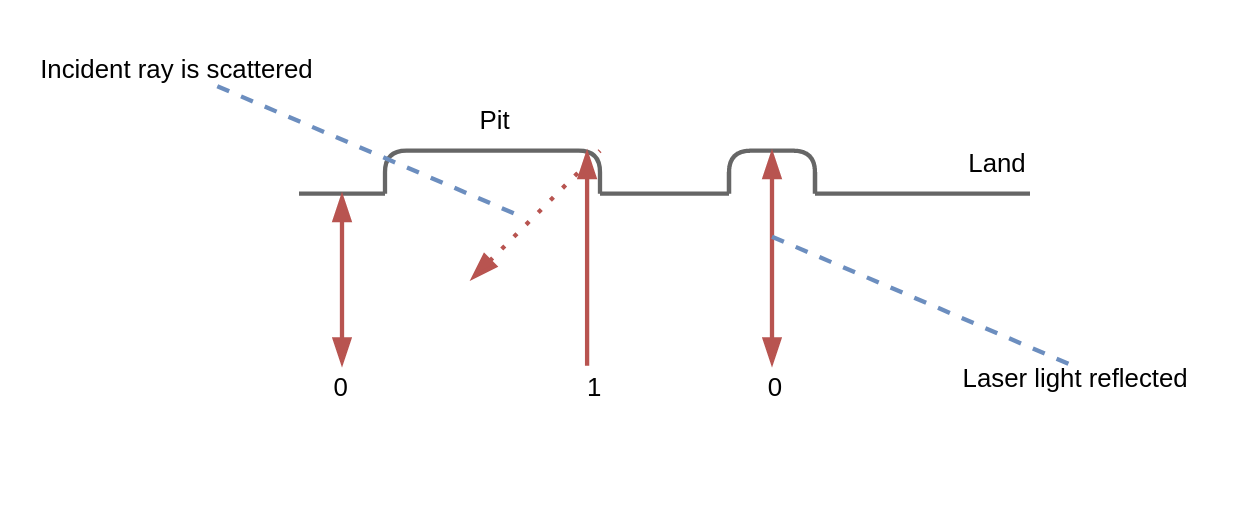
\includegraphics[width=0.9\textwidth,keepaspectratio, frame]{./images/optical_disk.png}
\caption{The pits and lands of an optical disk}
\end{figure}

\textbf{Description:}

During manufacturing, intense laser light is reflected onto a \emph{CD-ROM} disk to burn pits along the \emph{track}. During playback, a laser of lower intensity is directed at the track as it spins. At the beginning or end of a depression, light is scattered and not reflected back to the sensor. An area like this represents a \emph{1}. When the laser falls on the middle of a pit or land, light is reflected back towards the sensor and a \emph{0} is detected.

A recordable disk is covered with a transparent dye. A high intensity laser can alter the reflective properties of the dye. As the CD is read, the changes in the property of the surface affect the amount of light reflected, rather than pits and lands.

Certain types of compact disk can be rewritten. A high powered laser heats and deforms the surface of the disk. A magnet is used in conjunction with the laser to set the state of the spot while it is being heated. Similarly a \emph{DVD-RW} uses a 'phase change alloy' which changes between \emph{amorphous} and \emph{crystalline} states under the power of the laser light.

\textbf{Performance:}

A typical \emph{CD-ROM}, the oldest type of optical storage can hold about 650-700 MB of data, while a modern \emph{Blu-Ray} disk can store upwards of 50 GB of data. As technology has improved, shorter wavelengths of light are used to read the disk. This means the size of pits and lands can be reduced and still read at the same apparent resolution. More pits and lands can fit on the same length of track and the spiral can be packed more closely, increasing the amount of track that can fit on a single disk.

\subsubsection{Solid State Drives}
\label{sec:orgc6cdc51}

A Solid State Drive \emph{(SSD)} is a modern type of secondary storage, frequently used in personal devices. There are two common implementations of \emph{EEPROM}, those which use \emph{NOR} logic and those which use \emph{NAND}. The latter technology is more widely used in mass storage, as the storage density is higher and the cost per unit of storage is lower.

\textbf{Components:}

\begin{itemize}
\item Page
\item Block
\item Control Gate
\item Floating Gate
\item Oxide Layer
\item Bitline
\item WordLine
\end{itemize}

\textbf{Diagram:}

\begin{figure}[H]
\centering
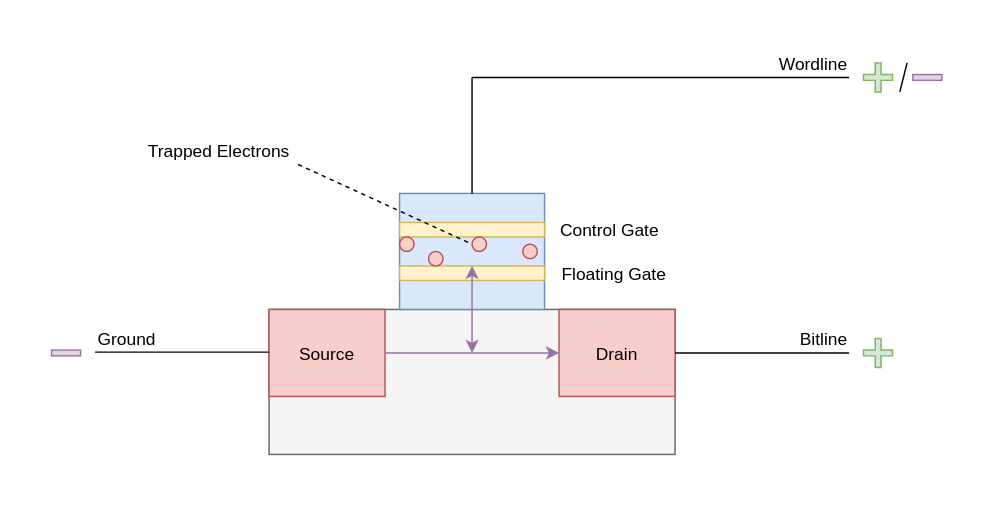
\includegraphics[width=0.9\textwidth,keepaspectratio, frame]{./images/nand_flash.png}
\caption{A nand cell}
\end{figure}

\textbf{Description:}

In order to retain information, a single nand cell contains two gates separated by \emph{oxide layers} which electrons cannot usually cross. As the \emph{bitline} is given a positive charge, electrons are drawn from the \emph{source} to the drain.

\begin{itemize}
\item If the \emph{wordline} is set to positive, some electrons are drawn up the oxide layers and trapped by the \emph{floating gate}
\item If the power is turned off, any trapped electrons remain in position
\item If the \emph{wordline} is set to negative, any electrons are forced out of the floating gate, clearing the cell
\end{itemize}

No charge in the trap is considered a \emph{1}, while any trapped electrons register a \emph{0}.

NAND memory divides storage into \emph{pages} and \emph{blocks}. It is not possible to overwrite existing pages using NAND technology and so a \emph{block} must be erased entirely if its constituent pages need to be modified. While it is possible to write data to a single page, it is not possible to \emph{erase} one page alone and so the whole block must be  backed up and cleared.

\textbf{Performance:}

The typical capacity of an \emph{SSD} is smaller than that of a \emph{HDD} and the price is generally higher per unit of storage. Solid state devices have the advantage of no moving parts, reducing the electrical power required and the space needed to install an SSD. This makes them useful in small mobile devices like phones and tablets, where space and battery power are limited. In addition, solid state devices are faster to read and write from as no seeking time is required; read-write heads do not have to be moved to a certain location before data can be read or written.

While the longevity of \emph{SSDs} is a topic of debate, they can be considered generally more reliable. The absence of moving parts reduces of the chance of the device suddenly failing, although the number of read write cycles is limited.

\section{Data Structures}
\label{sec:org2b3e3c0}

\emph{not implemented}

\section{Algorithms}
\label{sec:orgb7fe2d2}

\emph{not implemented}

\section{Regular languages}
\label{sec:org0a973f3}

\emph{not implemented}

\section{Communication Technology and Consequences}
\label{sec:org2d052ff}
\subsection{Communication Methods}
\label{sec:org35bf0c2}
\subsubsection{Serial Transmission}
\label{sec:org7e1cbd0}

During serial data transmission, bits are set one after the other down a single (serial) data channel. A second data wire will be needed for simultaneous bi-directional data transfer. Sometimes an additional \emph{ground} wire is used to reduce the adverse affects of interference. Additional control wires may also be used in serial data connections.

\subsubsection{Parallel Transmission}
\label{sec:org00ba9fd}

Multiple bits of data are sent simultaneously along a number of parallel data wires.

\subsubsection{Comparison of Methods}
\label{sec:orgcb71668}

Each of the wires used to transmit individual bits in a parallel connection will differ slightly from the others. This subtle difference will affect the rate at which data can travel along the wire and hence the time taken for a bit to travel a certain distance. This causes bits to arrive at the receiver at different times, a phenomena know as \emph{skew}.

Parallel transmission becomes impractical over larger distances, as \emph{skew} becomes more pronounced. Parallel transmission is, however, suitable in some environments, for example onboard motherboards and \emph{Integrated Circuits}, where distances are small and the increased speed is valuable.

Serial connections have much smaller interfaces, making them suitable for mass manufacturing, especially in mobile devices and consumer electronics.

\emph{Crosstalk} between the data channels of a parallel connection can cause interference and corruption. The danger of interference due to crosstalk increases with frequency. As a result, the frequency of serial connections can be safely increased beyond the practical limits of parallel connections, meaning more data can be transmitted in a given amount of time, even if less data is transferred per cycle.

\subsubsection{Bit and Baud Rate}
\label{sec:orgafd00ea}

The two measures are linked with this equation:

\emph{bit rate = baud rate * number of bits per baud}

In typical serial connections, \emph{1s} and \emph{0s} are represented by high and low voltages in a cable, called non-return-to-zero \emph{(NRZ)} communication, where the signal voltage never returns to \emph{0v}. The \emph{baud rate} is the number of symbol changes per second - the number of times the signal voltage is changed / the frequency. The bit rate may be the same as the \emph{baud rate}, although - using signal modulation - more than 2 values may be encoded within a single cycle. In such a case, the \emph{bit rate} (the total number of bits transferred in a second) is equal to the \emph{baud rate} * the number of bits per \emph{baud}.

Increasing the number of bits per \emph{baud} means more data can be transferred along a narrower (possibly serial) cable in a certain amount of time.

\subsubsection{Baseband and Broadband}
\label{sec:org4a89946}

Broadband is an analogue data transfer method, meaning there are a \emph{continuous} range of values (voltages) and each symbol change can represent more than two values (as in binary). Broadband connections are often multi-channel and bidirectional. These connections are frequently use in \emph{WANs}.

Baseband is a type of digital data connection, commonly used in \emph{LANs}, where the bit rate is often the same as the baud rate, hence each symbol is either a 0 or 1. Ethernet cables are baseband connections.

\subsubsection{Latency and Bandwidth}
\label{sec:orgf8c0882}

Latency is the time taken for some data to be transmitted a certain distance, ie. from sender to receiver, irrespective of how much data is sent at once. Latency is often measured in seconds \emph{(s)} or milliseconds \emph{(ms)}.

Bandwidth loosely means how much data can be received at once, irrespective of the speed the signal can travel and hence the latency between sender and receiver. Bandwidth is often measured in bits per second \emph{(bps)} and has a direct relationship to bit rate.

In data communication and networking, bandwidth is analogous to data transfer rate.

\subsubsection{Synchronous Communication}
\label{sec:orgfaba28e}

During \emph{synchronous transmission}, both sender and receiver share a common clock cycle for coordinating signals. This communication method depends on that clock cycle to govern communication along the wire. This type of communication is best for connections that work in real time, with a constant flow of data, for example within a computer's processor.

\subsubsection{Asynchronous Communication}
\label{sec:org55e577a}

There is another common communication method known as \emph{asynchronous transmission}. Neither the sender, nor the receiver share the same clock cycles. Communication is governed by start and stop bits, sent before and after a communique. The stop bit is always the opposite of the start bit. Despite the absence of a common clock, the sender and receiver must use the same baud/bit rate so that the receiver can understand the message once the start bit is received.

\subsection{Network Topology}
\label{sec:orge0b0405}

A single computer with no connection to any other devices is described as a \emph{stand-alone} computer system. When a computer is connected to one or more other computers, the resulting system can be described as a \emph{computer network}. Digital \emph{baseband} connections are often used inside a \emph{local area network}. Many smaller LANs spread over a large area are often joined to others by \emph{broadband} connections, creating a \emph{wide area network}.

\emph{Physical} network topology defines how the devices are physically connected with hardware devices and equipment. \emph{Logical} network topology is the layout used by devices on a network to communicate using the physical network equipment provided.

\subsubsection{Physical Bus Topology}
\label{sec:org946d4a6}

The \emph{physical bus topology} is a simple network configuration, used in many small home networks. Each device is connected to a \emph{backbone} cable which runs past every device. A \emph{terminator} is placed at either end of the bus.

\textbf{Advantages:}

\begin{itemize}
\item A bus network is inexpensive to set up and easy to maintain.
\item Less cable has to be laid/installed.
\item Identifying problems with equipment can be easier.
\end{itemize}

\textbf{Disadvantages:}

\begin{itemize}
\item Data intended for one device on the network passes many other computers.
\item The single backbone cable is subject to congestion as many devices need to communicate through the network.
\item Collisions can occur as devices need to send data along on the bus.
\item The single backbone cable is a single point of failure. If it is not functioning, it is impossible for devices on the network to communicate with one another.
\end{itemize}

\subsubsection{Physical Star Topology}
\label{sec:org9080515}

The \emph{physical star} network configuration is a more complicated type of network, where each node has its own dedicated connection to the hub or router.

\textbf{Advantages:}

\begin{itemize}
\item The star network is more secure, as data intended for one computer on the network does not pass by others.
\item Dedicated cables for each device eliminate the risk of collisions between signals sent by different computers.
\item This type of network is more flexible and expandable, as more hubs and devices can be connected to the hub.
\end{itemize}

\textbf{Disadvantages:}

\begin{itemize}
\item Star networks can be more difficult and expensive to implement as more cables need to be laid/installed.
\item The central hub is a single point of failure. Should the hub fail, none of the devices on the network will be able to communicate with one another.
\end{itemize}

\subsubsection{Logical Topology}
\label{sec:org9851270}

Logical topology is the manner in which data is handled on top of a physical network. For example, a hub might use a bus protocol to push data outward onto a star network, similar to how a physical bus network behaves.

\subsubsection{MAC Addresses}
\label{sec:orgf018ddc}
\subsection{Client/Server}
\label{sec:org66ca71a}

A \emph{server} is a computer which services requests from a number of clients; a response is sent back to the connected client in return. A computer may be both a client and a server simultaneously. A server might be used to process or store data.

Within a LAN, server(s) may be set-up to handle tasks common among all client computers on the network. Internet facing \emph{web-servers} are used to host websites and content on the internet.

\textbf{Advantages:}

A client-server configuration is preferred when central management over the whole network is needed, making this model popular in schools and businesses. Servers might be set up to handle user accounts, store files and manage backups.

\textbf{Disadvantages:}

A client-server network requires expensive hardware (the servers themselves) and personnel to maintain the servers. This makes the client-server model impractical on smaller home networks.

\subsection{Peer-to-peer}
\label{sec:org33d9168}

There is less core infrastructure in a decentralised peer-to-peer network. The services that would be provided by servers are shared amongst the clients.

\textbf{Advantages:}

No expensive server computers are required. Expertise and maintenance are not required on a peer-to-peer network.

\textbf{Disadvantages:}

All clients must be connected and powered-on for the network to function as expected. Peer-to-peer networking may leave a user's files visible to other devices on the network.

\subsection{Wireless Networking}
\label{sec:org8fa2a8d}
\subsubsection{Wi-Fi}
\label{sec:org63f348f}

\emph{Wi-Fi}, standing for \emph{wireless fidelity}, is a type of wireless network standard designed to be interoperable with \emph{IEEE 802.11} protocol and work alongside Ethernet at the \emph{Network Access} layer. Devices using wi-fi can connect to a \emph{wireless access point} and communicate with any other device on the network.

\subsubsection{NIC}
\label{sec:orga166b1d}

In order to connect to a wireless network, a device must have a wireless network interface card \emph{(NIC)}, a device will have a similar card for all its other interfaces, eg. Ethernet. The NIC has a hardcoded MAC address. The combination of an NIC and a computer is called a \emph{station}.

\subsubsection{SSID}
\label{sec:org272c489}

A service set identifier \emph{(SSID)} is a human readable name for a wireless network. It may be broadcast to devices within range of a \emph{WAP}, or kept private.

\subsubsection{Security}
\label{sec:org9e76662}

Any device within range of a \emph{WAP} could connect to an unprotected wireless network. A network password is often used in wi-fi protected access \emph{(WPA)} networks. \emph{WPA2} is also a common standard. A network owner may also choose to set up a MAC whitelist for ultimate control over which devices may connect. In order to connect, the MAC address of a computer's NIC must be added to the whitelist.

\subsubsection{CSMA/CA}
\label{sec:orgecfd985}

Connected devices share the same channel to transmit data to the \emph{WAP}. In order to prevent multiple computers trying to communicate with the \emph{WAP} simultaneously, Carrier Sense Multiple Access with Collision Avoidance \emph{(CSMA/CA)} is used. Before data may be sent to the \emph{WAP}, the station checks if the channel is idle. If another device is communicating over the channel, the station waits a random amount of time before checking the status of the channel again. This process continues until the channel is free and the station is able to send data to the \emph{WAP}.

\subsubsection{RTS/CTS}
\label{sec:org4e38311}

One of the shortcomings of the \emph{CSMA/CA} standard is the \emph{hidden node} problem. It is possible that the \emph{WAP} is engaged with a station that cannot be seen or heard by a station that needs to send data. This situation is common on larger networks, where the \emph{WAP} serves a larger area.

Once the channel appears idle to a station, a 'request to send' signal is sent to the \emph{WAP}. If the 'clear to send' signal is not received, the station waits a random amount of time before checking the channel status and resending the 'request to send' signal. If the \emph{WAP} is free, a 'clear to send' signal is returned to the station and the data can be transmitted.

\subsection{Communication \& Privacy}
\label{sec:org45820f1}

\emph{not implemented}

\subsection{Social, Cultural \& Legal Issues}
\label{sec:orgc73563d}

\emph{not implemented}

\section{The Internet}
\label{sec:org6507fe6}


The \emph{Internet Protocol Suite}, often referred to as the \emph{TCP/IP} stack, is a collection of communication protocols adopted on the public internet and other similar computer networks. The whole protocol suite governs end-to-end communication between devices including stipulations about the way data is split into packets, addressed transmitted and routed. Much like the \emph{Open Systems Interconnection}, these conceptual network models arrange communication protocols into abstract layers.

\subsection{Uniform Resource Locators}
\label{sec:org795772f}

A URL is a specific type of \emph{Uniform Resource Identifier} or URI, designed to identify web resources on computer networks. A typical URL may resemble:

\begin{verbatim}
https://www.example.com:443/path?query
\end{verbatim}

In the example above the \textbf{https} protocol is used, followed by the characters \texttt{://}. This whole component of the URL is called the \emph{scheme}. The next component is the host name or IP address, separated from the port number by a colon. The remaining components are the path to the resource or file in question and the query string, separated by a question mark.

\subsection{Domain Names \& DNS}
\label{sec:org0dd89b5}

A domain is an identification string which defines or identifies a \emph{``realm of administrative autonomy, authority or control''} within the internet (Wikipedia). Domain names conform to the rules and regulations of the \emph{Domain Name System}, which maps a domain to other types of information, such as an IP address. Any such string registered in the \textbf{DNS} is considered a domain name.

Domain names are organised, or grouped, in subordinate divisions of the domain root, which is nameless (refer to \textbf{FQDN}). The first level of domains are called \emph{top-level-domains} or \textbf{TLDs} for short. \textbf{TLDs} include generic top-level domains such as \texttt{com}, \texttt{info}, \texttt{net}, \texttt{edu}, and \texttt{org} as well as the country code top-level domains. Below this tier are the second and third-level domains. These are openly available for reservation to internet users. Domain names work from right to left, with the top-level domain appearing on the right. Domain levels are separated with the \texttt{.} (full stop) character.

\begin{itemize}
\item A \emph{fully qualified domain name} is all the components of a domain name, which collectively specify the domain's exact location in the domain name system. \textbf{FQDNs} are terminated with a full stop, which is characteristic of this type of domain. The point represents the root domain, from which the domain can be located.

\item A \emph{subdomain} is federated by the owner of the parent domain. There is no limit to how many subdomains may be used. Third-level domains are often used to identify a particular host server, eg \emph{mail} or \emph{www}. Such subdomains may only support the implied functionality.
\end{itemize}

The \emph{Internet Corporation for Assigned Names and Numbers} (ICANN) is the governing body for the name and number systems used on the internet. There are five \emph{Regional Internet Registries} globally. Registries are organisations which manage top-level domains. Through a memorandum of understanding, these registries cooperate through the unincorporated \emph{Number Resource Organisation}. Internet resources are distributed to RIRs and disseminated in accordance with the policies of the registry. The commercial sales of domain names are delegated to accredited \emph{internet registrars}. When a customer purchases, or more accurately \emph{leases}, a domain, the registrar notifies the registry which maintains the records. Regional registries allocate blocks of IP addresses to local internet registries, most often internet service providers.

\subsection{Protocol Stack}
\label{sec:org0775c31}

The internet protocol suite is a layered model, in which transmitted data descends through the layers as it is sent. This process is reversed when the data is received. At each layer, the data is further encapsulated in accordance with the workings of the lower-level protocol. The data handled at each layer is sometimes referred to as the \emph{Protocol Datagram Unit} (PDU). Each layer communicates with the layers immediately adjacent to itself, either the layer above or below during operation.

\begin{itemize}
\item \textbf{Application Layer:} contains abstract communication protocols used in process-to-process communication over an Internet Protocol (IP) network.

\item \textbf{Transport Layer:} responsible for device-to-device (or end-to-end) communication for applications. This layer facilitates connection-orientated communication (TCP) or best-effort stateless communication (UDP). The PDU for the transport layer is the \emph{segment} for TCP and the \emph{datagram} for UDP.

\item \textbf{Network Layer:} responsible for inter-network communication through network gateways. The PDU of the network layer is the IP packet. The protocols working at this level, most notably IP, are not connection orientated themselves, although can respond to transport layer service requests to provide such a system.

\item \textbf{Link Layer:} communication protocols limited to the physical connections of the current node within the same network segment. The link layer PDU is called a \emph{frame}.
\end{itemize}

\subsection{IP Addresses}
\label{sec:orge07cad9}

An \emph{Internet Protocol} address is a unique number assigned to a network interface involved in internet communication. The address identifies and locates the host, which allows a path to the host to be established. IPv4 is a 32-bit standard, although such small addresses have caused IP address shortages. To address this IPv6 addresses are 128 bits in length, offering many more addresses. A single IP address must be unique within a particular network, though the same address may be used on two separate networks.

The first portion of an address refers to the network, while the remaining bits are used to identify specific devices. Classful addressing was used to separate the network and host sections of a given address. The table below summarises how many bits were used in class A, B and C addressing. Class D was used for multicast addressing and class E was used for reserved addresses.

\begin{center}
\begin{tabular}{lr}
\hline
Class & Network Bits\\
\hline
A & 8\\
B & 16\\
C & 24\\
\hline
\end{tabular}
\end{center}

Classful addressing has been superseded by CIDR notation, where the number of bits in the host portion is appended onto the IP address after a forward slash, for example: \texttt{103.27.104.92/24}. This value can be used to determine of the subnet mask, which can be applied to the IP address with a logical AND operation to reveal the network portion. The subnet mask is a 32 bit number containing 1s in what would be the network portion of the address.

Large networks are often divided into smaller subnets for ease of operation and performance. Administration is made easier by reducing the broadcast domain of a single device on a network.

\subsection{Local Networks}
\label{sec:orgd350329}

The rapid consumption of available addresses that afflicts the 32-bit IPv4 system has been slowed by the uptake of private, non-routable addresses in local networks. These addresses must remain unique within the local network, although there is no expectation that these addresses are globally unique, they may be reused on another network. As a result, acquiring a private IP address does not involve an internet registry. Communication between two devices on different networks requires another system, called \emph{Network Address Translation} (NAT).

\emph{Dynamic Host Configuration Protocol} automatically provides IP information to devices on a network. This includes the allocation of an IP address and networking information such as the subnet mask. IP addresses may be allocated \emph{dynamically}, whereby one device may receive any address from the pool of available addresses and be subject to a changing address, or by \emph{static} reservation, where a single device permanently uses the same private IP address.

If a device inside one network with a private IP address needs to communicate with a device on the public internet, its private IP address is replaced with the public IP address of the network gateway. Any response to the outgoing communication will reach the network router, which recorded ongoing communications in a translation table. Using this information, the publicly routable address is replaced with the private IP address of the correct device.

To allow devices outside a particular network access to a server operating within, \emph{port forwarding} rules are configured on the network router. The firewall maps incoming requests on specified ports to devices within the network.

\section{Databases and Software Development}
\label{sec:org1eac048}
\subsection{Introduction to Databases}
\label{sec:org18d84e9}

The purpose of any database is to store data in the most intuitive manner possible, minimising the required disk space and delivering the most performant system. The Relational Database Management System \emph{(RDBMS)} has become a popular database paradigm, although some others exist. A \emph{RDBMS} is based on entity modelling and the relationships between entities.

\subsection{Database Systems Overview}
\label{sec:org045d104}

In production, applications like \emph{mysql} or \emph{mariadb} are used. These are two examples of a \emph{RDBMS}. A database server tends to run as a service in the background. It is usually possible to connect to a running database server, either locally or remotely, through the database console. Within the \emph{container database}, the individual databases are found. Each database is composed of \emph{tables} and information can be retrieved from one or many of these tables during a \emph{query}.

In the \emph{RDBMS} paradigm, each \emph{entity} within a dataset is represented with a \emph{table}. A table will have pre-defined \emph{columns}, one for each \emph{attribute} an entity has. Rows in a table are called \emph{records}, where one record represents one instance of an entity within a dataset. Each record has many \emph{fields}, filled with the data corresponding to each \emph{attribute} of the entity.

Every record in a table must be uniquely identifiable. A selection of columns, used together, will constitute the \emph{primary key} (all the data needed to select exactly one record from a table). It is possible that a record can be identified with the value of just one column. When the values held by multiple columns are needed, this is described as a \emph{composite key}. On an entity level, the information needed to identify an instance is called the \emph{entity identifier.}

\subsection{Relationships}
\label{sec:orga1cd30d}

Not only do entities have attributes, they also have relationships with other entities. Sometimes these relationships are logical, apparent within the data, while other times they are created to model data within the constraints of a \emph{RDMS}. When such an entity is created it can usually be traced back to some abstract entity like a seat on a flight, a job listing or a sale in a shop.

The three types of relationships are:

\begin{itemize}
\item \emph{one-to-one}
\item \emph{one-to-many}
\item \emph{many-to-many}
\end{itemize}

When one record maps to more than one other record, this is a \emph{one-to-many} relationship. The term \emph{many-to-one} is never used as its meaning is similar to \emph{one-to-many} while relationships expressed like \emph{many-to-one} rarely make sense in the real world.

A \emph{many-to-many} relationship can often be problematic, especially in a \emph{RDMS}. in order to reduce repetition within a database, a transaction table is usually built between tables with such a relationship. This reduces the \emph{many-to-many} into two \emph{one-to-many} relationships. The resulting transaction table will usually have a composite key, constituted by the foreign keys of the two records that are being linked. Seeing as this is the intended purpose of the table, a separate identifier is not usually required.

\subsection{Normalisation}
\label{sec:orgc28cc49}

In order to reduce data duplication and make insightful queries easier to construct, there are some rules to follow. These rules dictate which \emph{normal form} a database is in. \emph{First normal form} is essential for most Database Management Systems \emph{DBMS}, while third normal form is ideal. The general rule is:

\emph{The data depends on the key (1nf), the whole key (2nf) and nothing but the key (3nf)}

\subsubsection{Un-normalised}
\label{sec:orgeb4482f}

\emph{There are many companies involved in the production of a modern airliner, this hypothetical dataset joins aircraft to the companies which make the engines (not on specification!).}

This table shows some data which is human-readable, but difficult to query. A major problem with this layout is the duplication of data. In a production database, this would significantly increase the size of the database and adversely affect performance. Data inconsistency is also a problem when the same data is stored more than once. In this table some fields have more than one value, which means the records are not uniquely addressable.


\begin{figure}[H]
\begin{center}
% \begin{longtable}{rlllllll}
\begin{longtable}{ |C{0.05\textwidth}|C{0.08\textwidth}|C{0.105\textwidth}|C{0.1\textwidth}|C{0.1\textwidth}|C{0.1\textwidth}|C{0.07\textwidth}|C{0.1\textwidth}| }

\hline
&&&&&&&\\
\textbf{id} & \textbf{name} & \textbf{price} & \textbf{engine \_id} & \textbf{engine \_name} & \textbf{engine\_ quantity} & \textbf{supplier \_id} & \textbf{supplier \_name}\\
&&&&&&&\\
\hline
&&&&&&&\\
123 & A320 & 100,000,000 & 1100G, 1A & geared turbofan, high bypass engine & 2, 2 & PW, CFM & Pratt \& Whitney, CFM International\\
&&&&&&&\\
\hline
&&&&&&&\\
243 & 737 & 100,000,000 & 1100G, 1B & geared turbofan, high bypass engine & 2, 2 & PW, CFM & Pratt \& Whitney, CFM International\\
&&&&&&&\\
\hline
&&&&&&&\\
156 & A380 & 400,000,000 & 900, 7000 & Trent 900, EA GP7000 & 4, 4 & RR, EA & Rolls Royce, Engine Alliance\\
&&&&&&&\\
\hline
&&&&&&&\\
457 & Typhoon & 110,000,000 & 2000 & EJ2000 & 2, 2 & RR & Rolls Royce\\
&&&&&&&\\
\hline
\end{longtable}
\end{center}
\end{figure}

\subsubsection{First Normal Form}
\label{sec:orgded40bb}

To achieve \emph{first normal form} each field must have only one \emph{atomic} value and each record must be unique. Each record also requires a unique key, whether that be composite or individual. In this case, the primary key for each row in the table is \texttt{id + component\_id}. The table below shows all the data from before in \emph{1nf}.

\begin{figure}[H]
\begin{center}
% \begin{longtable}{rlllllll}
\begin{longtable}{ |C{0.05\textwidth}|C{0.08\textwidth}|C{0.105\textwidth}|C{0.1\textwidth}|C{0.1\textwidth}|C{0.1\textwidth}|C{0.07\textwidth}|C{0.1\textwidth}| }
\hline
&&&&&&&\\
\textbf{id} & \textbf{name} & \textbf{price} & \textbf{engine \_id} & \textbf{engine \_name} & \textbf{engine\_ quantity} & \textbf{supplier \_id} & \textbf{supplier \_name}\\
&&&&&&&\\
\hline
&&&&&&&\\
123 & A320 & 100,000,000 & 1100G & geared turbofan & 2 & PW & Pratt \& Whitney\\
&&&&&&&\\
\hline
&&&&&&&\\
123 & A320 & 100,000,000 & 1A & high bypass engine & 2 & CFM & CFM International\\
&&&&&&&\\
\hline
&&&&&&&\\
243 & 737 & 100,000,000 & 1100G & geared turbofan & 2 & PW & Pratt \& Whitney\\
&&&&&&&\\
\hline
&&&&&&&\\
243 & 737 & 100,000,000 & 1B & high bypass engine & 2 & CFM & CFM International\\
&&&&&&&\\
\hline
&&&&&&&\\
156 & A380 & 400,000,000 & 900 & Trent 900 & 4 & RR & Rolls Royce\\
&&&&&&&\\
\hline
&&&&&&&\\
156 & A380 & 400,000,000 & 7000 & EA GP7000 & 4 & EA & Engine Alliance\\
&&&&&&&\\
\hline
&&&&&&&\\
457 & Typhoon & 110,000,000 & 2000 & EJ2000 & 2 & RR & Rolls Royce\\
&&&&&&&\\
\hline
\end{longtable}
\end{center}
\end{figure}

\subsubsection{Second Normal Form}
\label{sec:org6f72260}

To satisfy \emph{second normal form} the data must meet  the criteria of \emph{1nf} and there must be no partial dependencies. A partial dependency can happen when a composite key is used. To make \emph{2nf} easy to achieve, relationships are often brought in here. To manage this, determine the separate entities in the data and create a table for each of them. By splitting up all the entities it is easier to make useful queries.

Relationships may be \emph{one-to-one}, \emph{one-to-many} (or vice-versa) or \emph{many-to-many}. Where a \emph{many-to-many} relationship exists, a transaction table is usually required, otherwise it is difficult to maintain the single field key needed for \emph{2NF}. Unlike regular entities, a transaction table usually represents something abstract, like a sale in a shop, a job listing or a seat on a flight.

\textbf{E.g.} In this database, add a transaction table like this:

\begin{figure}[H]
\begin{minted}[ frame=single, framesep=8mm, rulecolor=RuleGray, baselinestretch=1.3, fontsize=\small, breaklines, fontfamily=tt]{text}
aircraft >----< engine

aircraft --< engine_option >-- engine
\end{minted}
\end{figure}

Here is how the entity tables will look:

\textbf{aircraft}

\begin{center}
\begin{tabular}{rll}
\hline
id & name & price\\
\hline
123 & A320 & 100,000,000\\
243 & 737 & 100,000,000\\
156 & A380 & 400,000,000\\
457 & Typhoon & 110,000,000\\
\hline
\end{tabular}
\end{center}

\textbf{engine}

\begin{center}
\begin{tabular}{llll}
\hline
id & name & supplier\_id & supplier\_name\\
\hline
1100G & geared turbofan & PW & Pratt \& Whitney\\
1A & high bypass engine & CFM & CFM International\\
1B & high bypass engine & CFM & CFM International\\
900 & Trent 900 & RR & Rolls Royce\\
7000 & EA GP7000 & EA & Engine Alliance\\
2000 & EJ2000 & RR & Rolls Royce\\
\hline
\end{tabular}
\end{center}

\textbf{engine\_option:}

This is the transaction table between the two tables. This table has a composite key of \texttt{aircraft\_id + engine\_id}. All the data in each record depends on the whole composite key. This table handles the multiple entries for each aircraft and engine, while avoiding partial dependencies.

\begin{center}
\begin{tabular}{rlr}
\hline
aircraft\_id & engine\_id & engine\_quantity\\
\hline
123 & 1100G & 2\\
123 & 1A & 2\\
243 & 1100G & 2\\
243 & 1B & 2\\
156 & 900 & 4\\
156 & 7000 & 4\\
457 & 2000 & 2\\
\hline
\end{tabular}
\end{center}

\subsubsection{Third Normal Form}
\label{sec:orgfd0a7a1}

For data to be in \emph{third normal form}, \emph{1nf} and \emph{2nf} need to be satisfied. In addition, data in a record may not have any \emph{non-key} dependency, sometimes called lateral dependency. \emph{2nf} already establishes the need to depend on the whole key, but \emph{3nf} means that a field may not depend on any other attribute in addition to the primary key. In this database, the engine \texttt{supplier\_name} depends on the engine's \texttt{id}, but it also depends on \texttt{supplier\_id}. These situations are a good indication that another entity can be found and a new table created. This was not a problem in \emph{2nf}, because a \texttt{supplier} has a less troublesome \emph{one-to-many} relationship with the engine's \texttt{id}.

Here is the relationship that can be identified:

\begin{figure}[H]
\begin{minted}[ frame=single, framesep=8mm, rulecolor=RuleGray, baselinestretch=1.3, fontsize=\small, breaklines, fontfamily=tt]{text}
supplier ----< engine
\end{minted}
\end{figure}

With this type of relation, no transaction table is needed, therefore the complete \emph{3nf} database looks like this:

\textbf{aircraft:}

\begin{center}
\begin{tabular}{rll}
\hline
id & name & price\\
\hline
123 & A320 & 100,000,000\\
243 & 737 & 100,000,000\\
156 & A380 & 400,000,000\\
457 & Typhoon & 110,000,000\\
\hline
\end{tabular}
\end{center}

\textbf{supplier:}

\begin{center}
\begin{tabular}{ll}
\hline
id & name\\
\hline
PW & Pratt \& Whitney\\
CFM & CFM International\\
CFM & CFM International\\
RR & Rolls Royce\\
EA & Engine Alliance\\
RR & Rolls Royce\\
\hline
\end{tabular}
\end{center}

\textbf{engine}

\begin{center}
\begin{tabular}{lll}
\hline
id & name & supplier\_id\\
\hline
1100G & geared turbofan & PW\\
1A & high bypass engine & CFM\\
1B & high bypass engine & CFM\\
900 & Trent 900 & RR\\
7000 & EA GP7000 & EA\\
2000 & EJ2000 & RR\\
\hline
\end{tabular}
\end{center}

\textbf{engine\_option:}

\begin{center}
\begin{tabular}{rlr}
\hline
aircraft\_id & engine\_id & engine\_quantity\\
\hline
123 & 1100G & 2\\
123 & 1A & 2\\
243 & 1100G & 2\\
243 & 1B & 2\\
156 & 900 & 4\\
156 & 7000 & 4\\
457 & 2000 & 2\\
\hline
\end{tabular}
\end{center}

\subsection{Diagrams}
\label{sec:org31c5a9f}

There are a number of different methods used to design and plan complicated database layouts. Some are visual, while others, like \emph{entity descriptions}, are not.

\subsubsection{Entity Descriptions}
\label{sec:org4d39562}

In an entity description, each line represents a table. The first section is the table name and then, within brackets, the attributes being implemented as columns. This vaguely resembles a SQL statement, although the data-types and constraints are missing. The key is underlined and any foreign keys are usually italicised.

\textbf{Example from Chat Application:}

\begin{itemize}
\item user (\_id\_, username, password, salt, last\_login)
\item chat\_user (\_user\_id, chat\_room\_id\_)
\item chat\_room (\_id\_, name, pin)
\item message (\_id\_,  text, time\_stamp, \emph{owner\_id}, \emph{chat\_room\_id})
\item attachment (\_id\_, path, time\_stamp, \emph{message\_id})
\end{itemize}

\subsubsection{Entity Relation Diagrams}
\label{sec:orgaf46a2e}

\emph{ER} diagrams are a more visual way of representing a database layout. There are two common types, those which include the table/entity name only and those which show the columns and foreign key relationships. Here are some examples:

\begin{figure}[H]
\centering
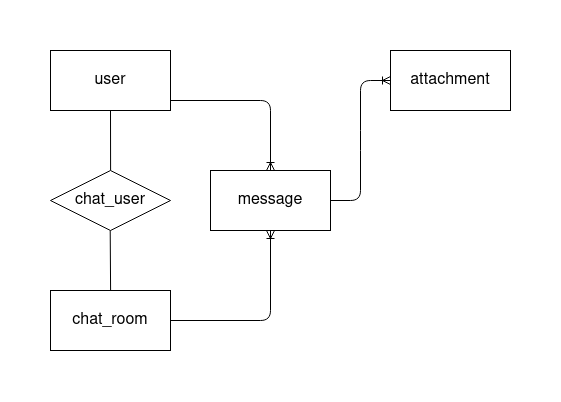
\includegraphics[width=0.7\textwidth,keepaspectratio, frame]{./images/er_simple.png}
\caption{An abstract entity relation diagram}
\end{figure}

\begin{figure}[H]
\centering
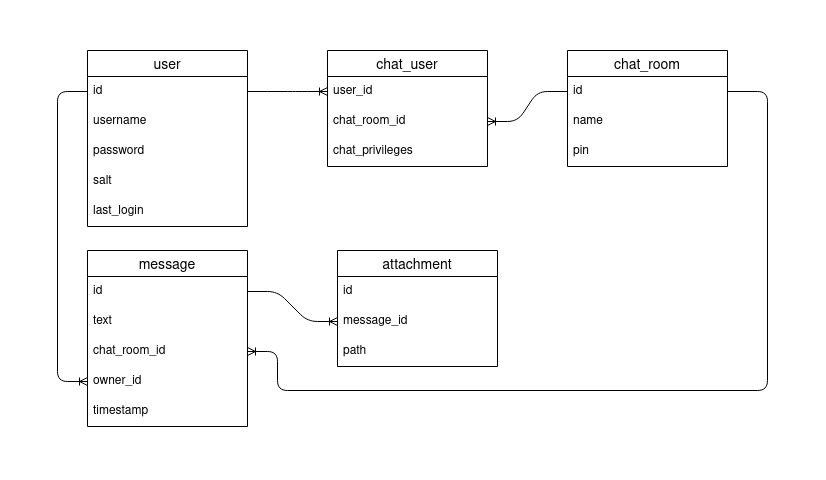
\includegraphics[width=0.9\textwidth,keepaspectratio, frame]{./images/er_complex.png}
\caption{A more detailed entity relation diagram}
\end{figure}


\subsection{SQL}
\label{sec:org7dde1cb}

SQL, standing for \emph{structured query language}, is a declarative, high-level language for manipulating and querying databases. There are a number of SQL compatible database programs, two common ones being MYSQL and Mariadb. Database administration and set-up are not required parts of the A-Level specification.

SQL commands are generally shown in uppercase, although in most implementations they are case-insensitive. A command can span multiple lines, white-space rarely matters and commands are finished with a semicolon.

\subsubsection{Creating Tables}
\label{sec:org1335339}

Assuming that a database has been set-up, the first step is to create the tables which will hold the data. As there are some foreign key relationships, it is important that the tables are created in the right order.

This example will use the db design from the normalisation example above, leaving some mistakes to be corrected later.

\begin{figure}[H]
\begin{minted}[ frame=single, framesep=8mm, rulecolor=RuleGray, baselinestretch=1.3, fontsize=\small, breaklines, fontfamily=tt]{sql}
CREATE TABLE aircraft (
    id INT(255) NOT NULL AUTO_INCREMENT,
    name VARCHAR(255),
    price FLOAT(24),
    PRIMARY KEY (id));

CREATE TABLE supplier (
    id VARCHAR(3) NOT NULL,
    name VARCHAR(255),
    PRIMARY KEY (id));

CREATE TABLE engine (
    id VARCHAR(10) NOT NULL,
    name VARCHAR(255),
    supplier_id VARCHAR(3),
    PRIMARY KEY (id));

CREATE TABLE engine_option (
    aircraft_id INT(255) NOT NULL,
    engine_id VARCHAR(10),
    FOREIGN KEY (aircraft_id) REFERENCES aircraft (id)
    ON DELETE CASCADE ON UPDATE CASCADE,
    FOREIGN KEY (engine_id) REFERENCES engine (id)
    ON DELETE CASCADE ON UPDATE CASCADE);
\end{minted}
\end{figure}

Notice that each column has a datatype, the number following each one represents the maximum display width or the precision in the case of \texttt{FLOAT}. The best information on these data-types is the official documentation: \url{https://dev.mysql.com/doc/refman/8.0/en/data-types.html}

\textbf{Extra Info:}

\begin{itemize}
\item Features like \emph{not null} and \emph{auto\_increment} are often used. Generally most columns are filled, although a column marked with \emph{not null} will cause an error if no value is assigned. The id column of one of the tables is set to \emph{auto\_increment}, so a unique id is generated if one is not explicitly provided.
\item Key constraints are used to manage the entity identifier within the database implementation. A \emph{foreign key} column must have the same datatype as the column being referenced.
\item The only notable data-type not shown in this db is a date/time format. They can be manipulated using the \texttt{<} and \texttt{>} symbols, making them very flexible. Additionally, \emph{timestamps} and \emph{datetime} fields can be updated with the current time automatically by the \emph{RDBMS}.
\end{itemize}

\textbf{Examining Tables:}

The list of tables can be shown and an individual table described with these commands respectively \emph{(not on specification)}:

\begin{figure}[H]
\begin{minted}[ frame=single, framesep=8mm, rulecolor=RuleGray, baselinestretch=1.3, fontsize=\small, breaklines, fontfamily=tt]{text}
show tables;
describe table_name;
\end{minted}
\end{figure}

\subsubsection{Altering Tables}
\label{sec:org6c3fa3e}

Once created, a table's definition may need to be changed. The \texttt{Alter Table} command is used for this.

Adding a constraint to a table is done like this (not on specification):

\begin{figure}[H]
\begin{minted}[ frame=single, framesep=8mm, rulecolor=RuleGray, baselinestretch=1.3, fontsize=\small, breaklines, fontfamily=tt]{sql}
ALTER TABLE engine ADD FOREIGN KEY (supplier_id) REFERENCES supplier (id) ON DELETE CASCADE ON UPDATE CASCADE;
\end{minted}
\end{figure}

Adding a column is also possible:

\begin{figure}[H]
\begin{minted}[ frame=single, framesep=8mm, rulecolor=RuleGray, baselinestretch=1.3, fontsize=\small, breaklines, fontfamily=tt]{sql}
ALTER TABLE engine_option ADD engine_quantity INT(1);
\end{minted}
\end{figure}

Existing columns can be renamed with ease:

\begin{figure}[H]
\begin{minted}[ frame=single, framesep=8mm, rulecolor=RuleGray, baselinestretch=1.3, fontsize=\small, breaklines, fontfamily=tt]{sql}
ALTER TABLE engine_option RENAME COLUMN engine_quantity TO engine_number;
\end{minted}
\end{figure}

The definition of a column can be modified:

\begin{figure}[H]
\begin{minted}[ frame=single, framesep=8mm, rulecolor=RuleGray, baselinestretch=1.3, fontsize=\small, breaklines, fontfamily=tt]{sql}
ALTER TABLE engine_option MODIFY COLUMN engine_number INT(255) NOT NULL;
\end{minted}
\end{figure}

Columns can also be dropped or deleted:

\begin{figure}[H]
\begin{minted}[ frame=single, framesep=8mm, rulecolor=RuleGray, baselinestretch=1.3, fontsize=\small, breaklines, fontfamily=tt]{sql}
ALTER TABLE engine_option DROP COLUMN engine_number;
\end{minted}
\end{figure}

\subsubsection{Inserting Data}
\label{sec:org02b713d}

The general syntax for a simple insertion is:

\begin{figure}[H]
\begin{minted}[ frame=single, framesep=8mm, rulecolor=RuleGray, baselinestretch=1.3, fontsize=\small, breaklines, fontfamily=tt]{sql}
INSERT INTO table_name (first_column_name, second_column_name) VALUES
    (first_value, second_value),
    (third_value, fourth_value);
\end{minted}
\end{figure}

Here are the insert statements for the aircraft demo:

\begin{figure}[H]
\begin{minted}[ frame=single, framesep=8mm, rulecolor=RuleGray, baselinestretch=1.3, fontsize=\small, breaklines, fontfamily=tt]{sql}
INSERT INTO supplier (id, name) VALUES
            ('PW', 'Pratt & Whitney'),
            ('CFM', 'CFM International'),
            ('RR', 'Rolls Royce'),
            ('EA', 'Engine Alliance');

INSERT INTO aircraft (id, name, price) VALUES
            (123, 'A320', 100000000),
            (243, '737', 100000000),
            (156, 'A380', 400000000),
            (457, 'Typhoon', 110000000);

INSERT INTO engine (id, name, supplier_id) VALUES
            ('1100G', 'geared turbofan', 'PW'),
            ('1A', 'high bypass engine', 'CFM'),
            ('1B', 'high bypass engine', 'CFM'),
            ('900', 'Trent 900', 'RR'),
            ('7000', 'EA GP7000', 'EA'),
            ('2000', 'EJ2000', 'RR');

INSERT INTO engine_option (aircraft_id, engine_id, engine_number) VALUES
            (123, '1100G', 2),
            (123, '1A', 2),
            (243, '1100G', 2),
            (243, '1B', 2),
            (156, '900', 4),
            (156, '7000', 4),
            (457, '2000', 2);
\end{minted}
\end{figure}

\subsubsection{Selecting Data (One Table)}
\label{sec:org12535d3}

Once there is some data in the database, organised in \emph{3nf}, it is possible to start making some queries to return records, using the \texttt{SELECT} statement.

The most simple query returns data from just one table. Here are some examples:

\begin{figure}[H]
\begin{minted}[ frame=single, framesep=8mm, rulecolor=RuleGray, baselinestretch=1.3, fontsize=\small, breaklines, fontfamily=tt]{sql}
SELECT * FROM aircraft;
SELECT name FROM supplier;
SELECT name, supplier_id FROM engine;
\end{minted}
\end{figure}

The first command returns the values from all columns of the \texttt{aircraft} table, while the others specify certain, comma-separated columns to display.

\subsubsection{Selecting Data (Multiple Tables)}
\label{sec:org13635bd}

There are a number of ways to select data from multiple tables, including \emph{joins} and \emph{sub-selects}, neither of which are on the a-level specification.

Here are some example queries across multiple tables:

\begin{figure}[H]
\begin{minted}[ frame=single, framesep=8mm, rulecolor=RuleGray, baselinestretch=1.3, fontsize=\small, breaklines, fontfamily=tt]{sql}
SELECT supplier.name, engine.name FROM supplier, engine WHERE supplier.id = engine.supplier_id;

SELECT supplier.name, engine.name FROM supplier, engine WHERE supplier.id = engine.supplier_id AND supplier.id = 'CFM';
\end{minted}
\end{figure}

Note that the \texttt{WHERE} clause provides the condition for the selection. In the second query, \texttt{AND} is used to provide a second condition.

\subsubsection{Ordering Results}
\label{sec:orgabf4b26}

The results of a select statement can be ordered in a certain way, using the \texttt{ORDER BY} statement. Here is an example:

\begin{figure}[H]
\begin{minted}[ frame=single, framesep=8mm, rulecolor=RuleGray, baselinestretch=1.3, fontsize=\small, breaklines, fontfamily=tt]{sql}
SELECT * FROM aircraft ORDER BY id DESC;
\end{minted}
\end{figure}

This will return all the results in order from highest id to lowest id. If the sort column is a string, the results will be sorted alphabetically. Multiple Columns can be specified as sort column, for example results might be sorted alphabetically by country and then city.

\subsubsection{Full Query}
\label{sec:org4af3ec5}

For a fully fledged database query, this is the default syntax:

\begin{figure}[H]
\begin{minted}[ frame=single, framesep=8mm, rulecolor=RuleGray, baselinestretch=1.3, fontsize=\small, breaklines, fontfamily=tt]{sql}
SELECT first_column_name, second_column_name
FROM first_table_name, second_table_name
WHERE first_condition AND second_condition
ORDER BY column_name DESC/ASC;
\end{minted}
\end{figure}

\subsubsection{Updating Records}
\label{sec:org9700831}

In addition to the table's definition, records can be changed. The \texttt{UPDATE} command is used to do this. Here are a few examples:

\begin{figure}[H]
\begin{minted}[ frame=single, framesep=8mm, rulecolor=RuleGray, baselinestretch=1.3, fontsize=\small, breaklines, fontfamily=tt]{sql}
UPDATE aircraft
SET name = 'a320'
WHERE id = 123;

UPDATE aircraft
SET price = price+20000000
WHERE id = 243;
\end{minted}
\end{figure}

Once again, the \texttt{WHERE} clause is used to supply the conditions for the statement.

\subsection{Client-Server Databases}
\label{sec:orgad256c9}

Many modern \emph{RDBMS} support a client-server model, where the database is stored on a central server and many clients can connect across the network. This is useful in retail, for example, where individual stores can access the same information about products, without the need for the data to be stored locally. Other benefits include the consistency of data, which can be guaranteed by storing it in one place only. In addition, the integrity of the data is upheld, as backups and access rights are managed centrally.

\subsubsection{Record Locking}
\label{sec:org03871b1}

If one client needs to modify a record, the encapsulating block of data is copied to the client workstation. Once the data has been modified, the block is submitted back to the central server.

If another client checked out the same block during this period, and resubmitted it after the first client had finished with the data, the second client may find that the block present in the server does not match the block it took out and modified. If the second client continued to submit its changes anyway, the update by the first client will be lost.

To solve this problem, \emph{record locking} was introduced, whereby a block being modified by a client cannot be accessed until it is returned to the server. This prevents simultaneous access completely, upholding the consistency of the data.

\subsubsection{Deadlock}
\label{sec:orgb8269bf}

The problem with \emph{record locking} is \emph{dead-lock}. It is possible that two different clients \emph{(1 \& 2)} have taken out different blocks of data \emph{(A \& B)} and now they both want to access the data held by the other client.

\begin{itemize}
\item Client 1 is holding \emph{block A} and waiting for \emph{block B}
\item Client 2 is holding \emph{block B} and waiting for \emph{block A}
\end{itemize}

Neither client returns the data and both wait for one another unknowingly. There are a number of techniques used to solve \emph{deadlock}.

\subsubsection{Serialisation \& Timestamp Ordering}
\label{sec:org778f666}

In order to prevent concurrent access, each record has two timestamps, \emph{read} and \emph{write} which are set whenever a transaction is applied. When a transaction begins it is also given a timestamp.

Whenever transactions need to be applied, the timestamps are checked and the transaction with the first timestamp is applied first. The timestamp of a transaction is compared against the timestamps of the affected records.

Using all of this information, the DB management software can apply transactions in the order they began and keep the data consistent.

\subsubsection{Commitment Ordering}
\label{sec:orgd29d4a2}

Commitment Ordering is another \emph{serialisation} technique, used to manage concurrent access. In addition to the time transactions were initialised, modifications are ordered by the dependencies on one another and the data stored in the DB.

\subsection{Approach to Problem Solving}
\label{sec:org8323c5d}
\subsubsection{Analysis}
\label{sec:orgcea444f}

Before development begins, the requirements of the client must be established. This includes identifying the shortcomings of existing solutions. Some of the factors to consider include the client's existing data and how it will be handled by the new system.

\subsubsection{Agile Modelling}
\label{sec:org98a8f21}

A large project is sometimes broken down into smaller parts like implementing a certain feature. During development, certain parts of the project may be developed at different rates.

The analysis of one feature may be concluded after the implementation of another. Developers may need to conduct a feasibility study, proving one requirement can be met, before continuing work on others. (feasibility study is no longer in specification)

Working with a client can be an \emph{iterative process}. The client will provide feedback regularly, as prototypes are built. This allows the program to be \emph{refined} as it is developed.

\subsubsection{Design}
\label{sec:org11dcc82}

After the requirements of the project have been finalised between the developers and the client, the developers can decide how the program will be made. Factors to consider include:

\begin{itemize}
\item input data
\item data structures
\item algorithms
\item output data
\item UI/UX
\item security
\item hardware requirements
\end{itemize}

\subsubsection{Implementation}
\label{sec:orgd8718e7}

During the implementation section, the requirements identified in the analysis section are met using the techniques outlined in the design phase. Whilst the features are being implemented, it is important to keep to the \emph{critical path}, the required features must be met before any others.

\subsubsection{Testing}
\label{sec:orge08d787}

All inputs are tested with normal, boundary and erroneous data. Other tests include:

\begin{itemize}
\item Unit testing
\item Module testing
\item Sub-system testing
\item System testing
\end{itemize}

Once the system is working, the client performs \emph{acceptance testing}, making sure that the system works with their data and meets their requirements.

Testing is also an \emph{iterative process}. Should the software fail the client's acceptance testing, for example, the developers may make some changes and run the new code through existing tests.

\subsubsection{Evaluation}
\label{sec:org9368fc6}

Three to six months after the delivery of the software, a post-implementation review may be conducted to determine the final quality and suitability of the system. The project may be judged on \emph{effectiveness}, \emph{usability} and \emph{maintainability} by the client. Thw review is a good opportunity to discuss improvements to the software.

\section{OOP and Functional Programming}
\label{sec:org250a0bf}
\subsection{Imperative Programming}
\label{sec:org1d77ead}

Early high-level languages fell into the \emph{imperative} category, meaning a program consisted of a series of steps, executed in order, to solve a problem. This paradigm developed naturally, as programs featured explicit steps for a computer to perform, in contrast to \emph{declarative} languages.

\subsection{Procedural Languages}
\label{sec:orgf7490fe}

Programs that divided these steps into separate functions and subroutines were called \emph{procedural} languages. The control flow of a procedural program follows a sequence of subroutine calls. Data in such programs is held separately in primitive types. Each piece of data exists in a certain scope, whether that is \emph{global} or \emph{local}, and data can be passed to a sub-routine as an argument.

Sub-routines can be divided into two types:

\begin{itemize}
\item \emph{procedures}, which may have parameters and return values, but also cause side-effects
\item \emph{functions}, which may have parameters and must have return values, while causing no side-effects
\end{itemize}

Many modern imperative languages support both types of sub-routine. \emph{Purely functional} languages are those which only support the latter, the benefits of which are explained in the functional programming section.

\subsection{Object Orientation}
\label{sec:orgb2330e8}

More modern programming languages associated data with behaviour, creating \emph{objects}. In an object orientated program, both real world data and program code are considered objects.

Here are some notes on how to use some of python's OOP features: \url{https://github.com/alexander-neville/docs/blob/main/python.org}

\subsubsection{Implementations of OOP}
\label{sec:org4e731d0}

Since \emph{OOP} is a paradigm, many languages support similar, although slightly different, programming techniques for working with types and objects. Generally speaking a named instance of a object is a \emph{reference type}, holding a pointer to where the object itself resides in memory.

\begin{figure}[H]
\centering
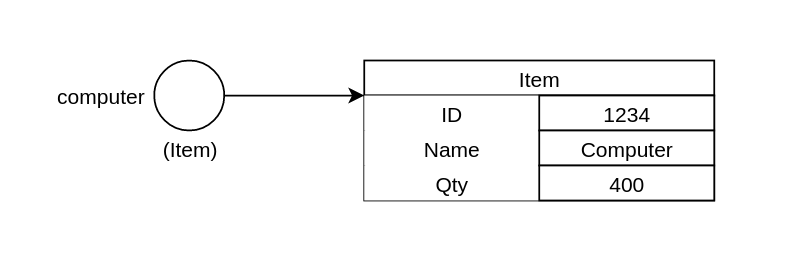
\includegraphics[width=0.9\textwidth,keepaspectratio, frame]{./images/reference.png}
\caption{Reference type}
\end{figure}

There are many different implementations of objects across different languages, from \emph{structs} in C and \emph{object literals} in Javascript to \emph{classes} in python and C++.

\subsubsection{Classes}
\label{sec:org2cb341c}

While it is possible to work in the object orientated style without classes, it is a useful construct pervasive in most OOP languages. A class is a blueprint for an object, defining the data and behaviour of an object.

Within the class for an object, certain attributes may be marked as \emph{private}, preventing the state being modified outside of the \emph{instantiated} object's own behaviours. So called \emph{information hiding} is an important improvement over traditional \emph{procedural} code, as it reduces \emph{mutability} and unexpected \emph{side-effects}.

This is an example of a class, written in pseudocode:

\begin{figure}[H]
\begin{minted}[ frame=single, framesep=8mm, rulecolor=RuleGray, baselinestretch=1.3, fontsize=\small, breaklines, fontfamily=tt]{text}
item = Class
    Public
        Function GetStockLevel
        Procedure UpdateStockLevel
        Procedure SellItem
        Procedure Describe
    Private
        Id: Integer
        StockLevel: Integer
        Name: String
        Description: String
End
\end{minted}
\end{figure}

Most attributes of the object are marked as private, while the object's behaviour is usually public. This is how other parts of the code interact with the object. Sometimes \emph{getter} and \emph{setter} methods are used to manipulate the attributes of a method. In this class, \texttt{GetStockLevel()} and \texttt{UpdateStockLevel()} perform this role.

\subsubsection{Encapsulation}
\label{sec:orga2cbaa4}

The association of data with behaviour, especially the use of \emph{getter} and \emph{setter} sub-routines, is called \emph{encapsulation}. By including the methods which operate on the data with the data itself, in a single object, access to the data from the program at large is restricted, hiding implantation details and better maintaining state across the program. Additionally, an interface can easily be built around the data, by modelling objects with classes, which makes the organisation of a larger project much simpler.

\subsubsection{Instantiation}
\label{sec:org54675e4}

A class may also include a \emph{constructor}, a sub-routine used to create an \emph{instance} of and object. This sub-routine is run when an object is \emph{instantiated} from a class. Each instantiated object has all the attributes and methods defined by the class. The precise value of each of these properties is associated with the instance, so it is possible to have many different instances of a single object. In most programming languages an instance is a reference type.

\subsubsection{Polymorphism}
\label{sec:org0c6a4ad}

Using a combination of object orientated techniques, a single \emph{interface} can be shared by a number of different objects (instantiated from different classes). This means that a single \emph{message} applied to a number of instances will cause a different action depending on the type of object receiving the message. For this technique to work, each object must implement some behaviour for the \emph{message}.

A \emph{message} is simply a call to an object's methods. For example:

\begin{figure}[H]
\begin{minted}[ frame=single, framesep=8mm, rulecolor=RuleGray, baselinestretch=1.3, fontsize=\small, breaklines, fontfamily=tt]{text}
object1.test_message(inputs)
object2.test_message(inputs)
\end{minted}
\end{figure}

If the program is \emph{polymorphic}, the same method (in this case '\texttt{test\_message}') can be called on both \texttt{object1} and \texttt{object2}, even if they are instantiated from different classes. The results will depend on the objects implementation of that \emph{message}. Note that the classes for these objects must define this behaviour. Therefore, the name of the methods and the call pattern are identical, but the contents of the method could be very different

There are many constructs, across programming languages, that are used for building an interface over many classes. One example is \emph{inheritance}, which is a object orientated technique in itself, while another is the use of an \emph{interface}.

\subsubsection{Interfaces}
\label{sec:org5e77985}

A programming interface stipulates the messages which a related class must respond to. The interface does not define any behaviour itself and the behaviour of each subclass for the messages does not need to be known.

This is how an interface would look in pseudocode:

\begin{figure}[H]
\begin{minted}[ frame=single, framesep=8mm, rulecolor=RuleGray, baselinestretch=1.3, fontsize=\small, breaklines, fontfamily=tt]{text}
Public interface BankAccount
    Procedure GetAccNum
    Procedure GetSortCode
    Function Withdraw (Amount)
    Function CalcInterest (TimePeriod)
End
\end{minted}
\end{figure}

The interface might be implemented like this (pseudocode example):

\begin{figure}[H]
\begin{minted}[ frame=single, framesep=8mm, rulecolor=RuleGray, baselinestretch=1.3, fontsize=\small, breaklines, fontfamily=tt]{text}
Class ReputableFirm implements BankAccount
    Public
        Procedure GetAccNum
        Procedure GetSortCode
        Function Withdraw (Amount)
        Function CalcInterest (TimePeriod)
    Private
        AccNum: Integer
        SortCode: Integer
        InterestRate: Float
        Balance: Double
End

LoanShark = Class implementing BankAccount
    Public
        Procedure GetAccNum
        Procedure GetSortCode
        Function Withdraw (Amount)
        Function CalcInterest (TimePeriod)
    Private
        AccNum: Integer
        SortCode: Integer
        InterestRate: Double
        Balance: Float
End
\end{minted}
\end{figure}

Note that both classes implement the same public functions (same definition and parameters), however some of the attributes of either class differ. For example, an account with a loan shark may have an extortionate amount of interest, hence the rate is stored as a \texttt{Double} rather than a \texttt{Float}. The subclasses are responsible for implementing the methods specified by the interface, however the details of that implementation are unique to the classes themselves.

\subsubsection{Inheritance}
\label{sec:org3db2903}

A plain \emph{interface} is more suitable for vaguely unrelated objects, whereas \emph{inheritance} is designed for objects with behaviour in common. If inheritance is a good option, it can be said that the objects have an \emph{``is a''} relationship. For example a cat \emph{is an} animal.

An object may \emph{inherit} from multiple other classes at once, or inherit from a single class which also inherited from another class in turn. A subclass has all the properties and methods of the superclass/parent class. With each level of inheritance, a subclass can do any of these things:

\begin{itemize}
\item add another method to those inherited from the parent class(es)
\item \emph{override} or change the behaviour of a certain inherited method entirely
\item modify inherited behaviour (make a call to parent's implementation of a method)
\end{itemize}

In some programming languages it is possible to define entirely abstract classes, which \emph{must} be inherited from ( an abstract class cannot be instantiated on its own). This differs from an \emph{interface} because the abstract class does implement some base behaviour.

Here is the example of inheritance from the textbook (pg 354):

\begin{figure}[H]
\begin{minted}[ frame=single, framesep=8mm, rulecolor=RuleGray, baselinestretch=1.3, fontsize=\small, breaklines, fontfamily=tt]{text}
Animal = Class
    Public
        Procedure MoveLeft
        Procedure MoveRight
    Protected
        Position: Integer
End

Cat = SubClass (Animal)
    Public
        Procedure MoveLeft (override)
        Procedure EatMouse
    Private
        Name: String
End
\end{minted}
\end{figure}


Each subclass which inherits from the \texttt{Animal} parent class will have all the methods of the parent class. In the \texttt{Cat} subclass, the \texttt{MoveLeft} method is \emph{overriden}, but the \texttt{MoveRight} method is not changed. This means that a cat object will move right in the same way as a generic animal if that message is sent to the object. The \texttt{Cat} object also adds the \texttt{EatMouse} method, which is specific to a cat. Here is a diagram of inheritance:

\begin{figure}[H]
\centering
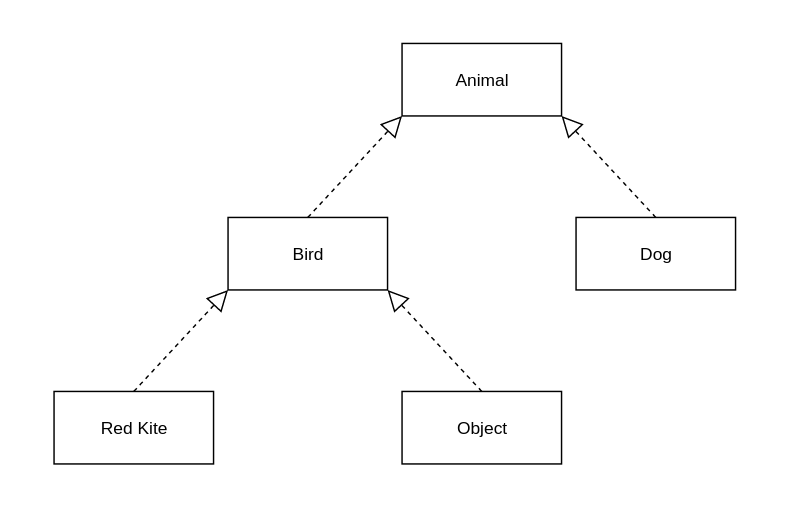
\includegraphics[width=0.9\textwidth,keepaspectratio, frame]{./images/inheritance.png}
\caption{Diagram of multiple inheritance}
\end{figure}

\subsubsection{Demonstration}
\label{sec:org9c4184d}

This is an example of inheritance and polymorphism written in python, but the theory is applicable to the a-level topic.

The first part of the program is the definition of the base class, in this case it is a model of an animal. This is not marked as abstract, but its role is parent class and its purpose is defining a standard interface and some default behaviour. For the sake of simplicity, the base class (and derived classes) only have one method in this example.

\begin{figure}[H]
\begin{minted}[ frame=single, framesep=8mm, rulecolor=RuleGray, baselinestretch=1.3, fontsize=\small, breaklines, fontfamily=tt]{python}
class Animal(object):


    def __init__(self):
        pass


    def describe(self):
        print("i am a generic animal")
\end{minted}
\end{figure}

With the base class established, two subclasses are defined, inheriting from the \texttt{Animal} class. These two classes model a bird and mammal respectively. They have more specific properties than the parent class and the \texttt{describe} method is overriden. The \texttt{Bird} class includes a call to the superclass' implementation of the message, as well as adding its own behaviour. In addition, the bird class has an additional property.

\begin{figure}[H]
\begin{minted}[ frame=single, framesep=8mm, rulecolor=RuleGray, baselinestretch=1.3, fontsize=\small, breaklines, fontfamily=tt]{python}
class Bird(Animal):


    def __init__(self):
        self.can_fly = True


    def describe(self):
        Animal.describe(self)
        print("i am a bird\n")



class Mammal(Animal):


    def __init__(self):
        pass


    def describe(self):
        print("i am a mammal\n")
\end{minted}
\end{figure}

A sub-routine is declared which can test the polymorphic design of the program. An instance object is passed to the sub-routine and the \texttt{describe()} method is called on the reference variable, irrespective of the object passed in. The outcome of the sub-routine will depend on the type of the object passed in, rather than the code in the sub-routine.

\begin{figure}[H]
\begin{minted}[ frame=single, framesep=8mm, rulecolor=RuleGray, baselinestretch=1.3, fontsize=\small, breaklines, fontfamily=tt]{python}
def test_object(animal):
    animal.describe()
\end{minted}
\end{figure}

The last part of the program is simply some driver code; two objects are instantiated and passed to the \texttt{test\_object()} sub-routine.

\begin{figure}[H]
\begin{minted}[ frame=single, framesep=8mm, rulecolor=RuleGray, baselinestretch=1.3, fontsize=\small, breaklines, fontfamily=tt]{python}
bird = Bird()
mammal = Mammal()

test_object(bird)
test_object(mammal)
\end{minted}
\end{figure}

The output succinctly demonstrates the principle of polymorphism. Both objects share a common interface, which can be called upon by an external unit of code. The resulting output is a consequence of the object's type, not the operation requested.

\begin{figure}[H]
\begin{minted}[ frame=single, framesep=8mm, rulecolor=RuleGray, baselinestretch=1.3, fontsize=\small, breaklines, fontfamily=tt]{text}
i am a generic animal
i am a bird

i am a mammal
\end{minted}
\end{figure}

\subsubsection{Association}
\label{sec:orgf36412b}

When two objects have a relationship that is not an \emph{``is a''} relationship, association by \emph{composition} or \emph{aggregation} may be more suitable. Such a relationship is usually a \emph{``has a''} relationship, for example a house \emph{has a} kitchen. There is usually some ownership involved, otherwise the objects can exist independently. The difference between the two types of association lies in the \emph{life cycle dependency} of the contained classes.

\begin{itemize}
\item during \emph{aggregation} association, the subclasses continue to exist without the container class, eg. people in a sports team or a company still exist if either is disbanded
\item during \emph{composition} association, the contained classes are destroyed along with the container class, eg. rooms in a building disappear if the building is knocked down
\end{itemize}

\begin{figure}[H]
\centering
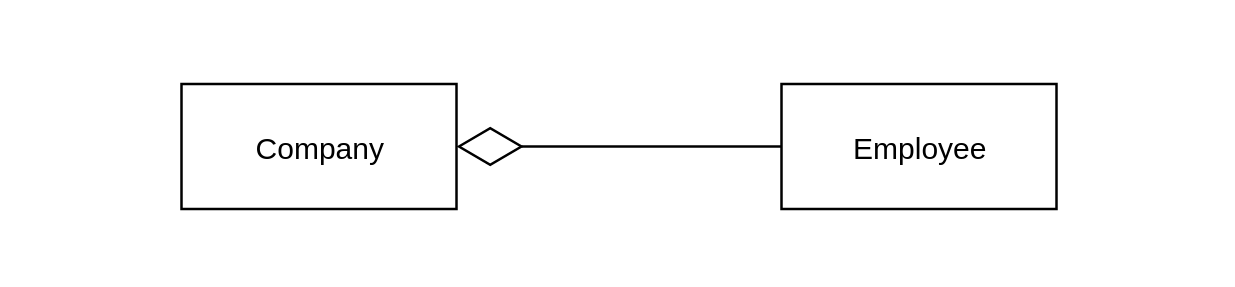
\includegraphics[width=0.9\textwidth,keepaspectratio, frame]{./images/aggregation.png}
\caption{Association by aggregation}
\end{figure}

\begin{figure}[H]
\centering
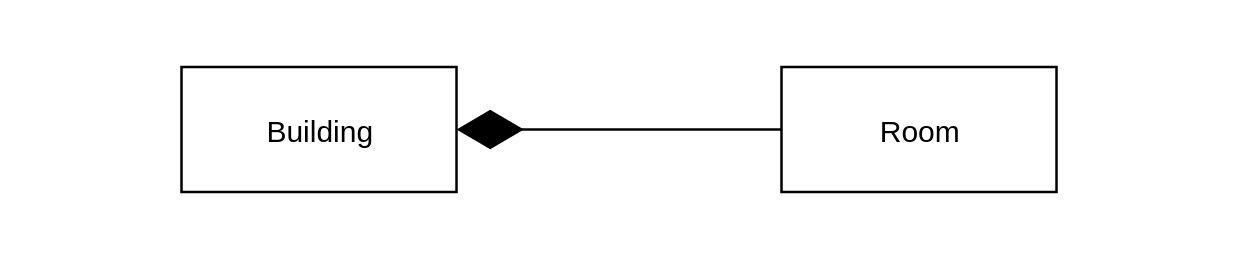
\includegraphics[width=0.9\textwidth,keepaspectratio, frame]{./images/composition.png}
\caption{Associaiton by composition}
\end{figure}

\subsubsection{Access Modifiers}
\label{sec:org0ada10a}

In programming languages, \emph{information hiding} can be enforced, so that program code must use an object's interface to retrieve data. There are generally three main modifiers:

\begin{itemize}
\item \emph{public} properties/methods can be used from anywhere in a codebase
\item \emph{private} properties/methods can only be accessed or run from within an object's own behaviours
\item \emph{protected} properties lie somewhere in between, depending on the language.
\end{itemize}

\subsubsection{Class Diagrams}
\label{sec:org659b578}

As is the case with DB design, there are a number of different diagrams designed to make working in the OOP style easier to plan. One common standard is the UML \emph{(unified modelling language)} diagram.

A single \texttt{-} sign is a private attribute, a \texttt{+} is a public attribute/method and \texttt{\#} is used for protected attributes.

\begin{figure}[htbp]
\centering
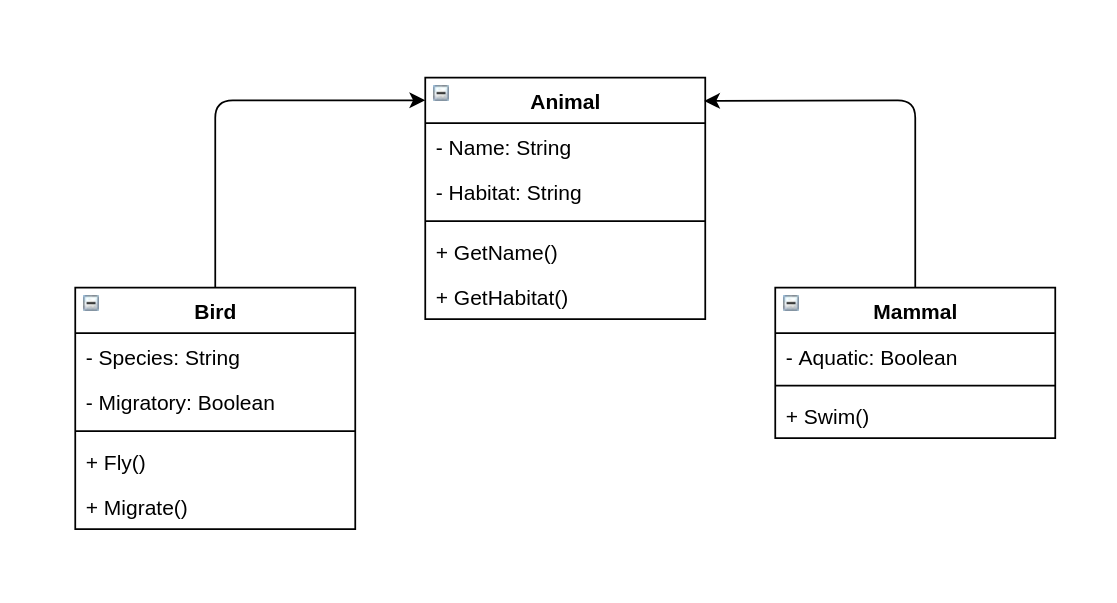
\includegraphics[width=.9\linewidth]{./images/uml.png}
\caption{A UML diagram for the standard animal example}
\end{figure}

\subsubsection{Advantages of OOP}
\label{sec:orgaf57bd7}

OOP is preferred to earlier procedural techniques for a number of reasons:

\begin{itemize}
\item planning is more important/worthwhile in the OOP paradigm
\item encapsulation means the implementation of data needs only happen once
\item an old OOP codebase is easily modifiable, by adjusting classes
\item general modularity and ease of debugging/maintenance
\end{itemize}

\subsection{Functional Programming}
\label{sec:org1ac7623}

\emph{not implemented}
\end{document}
